

% Code settings
\lstset{
  language=Scala, % C, C++, Java, SQL are from the around hundred available
  basicstyle=\ttfamily,
  numbers=left,
  numberstyle=\footnotesize,
  stepnumber=1,
  numbersep=2.0mm}



\chapter{SCOUt} \label{ch:scout}
This project explores the reliability and flexibility of using a single intelligent controller to complete exploration-based operations in diverse environments.
The Surveillance Coordination and Operation Utility (SCOUt) is used to generalize environments, agents, states and actions into abstract data structures.
This data then builds a platform for creating controllers, running simulations, and visualizing outputs.



% ==============================================================================
% Framework
% ==============================================================================
\section{Framework} \label{sec:framework}
Several coding languages and libraries are used in this project to provide a simple and expandable framework.
It is laid out in a client-server architecture (figure~\ref{fig:client_server_architecture}) to allow separation of data handling and data visualization.
The server portion provides full functionality to generate unique environments, build agents and controllers, run test operations, and collect results.
Data structures on the server side are implemented using an object-oriented architecture of traits, classes and class instances.
Traits are abstract objects that can be inherited by multiple classes.
Each class that inherits a trait can add specific values and behaviors to the object.
All classes that inherit from the same trait can be handled using the same logic, yet each class can behave in a unique way.
Different instances of a class can then be declared for repeated usage within code.
This data architecture was chosen to give the SCOUt framework simple extendibility into future projects.
The client is a graphical user interface (GUI) for requesting actions to be executed by the server and visualizing the data structures returned.
Because the majority of the data structures used in this platform are abstracted, the front end can be generalized to handle any new classes created without any maintenance required for the GUI.

\begin{figure}[!htb]
  \centering
  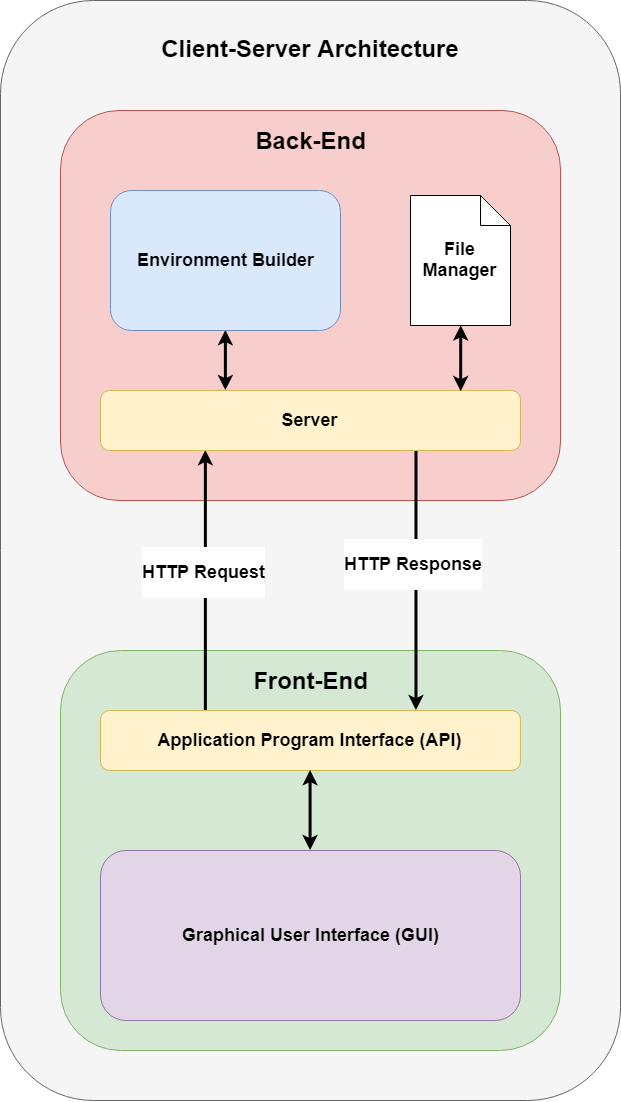
\includegraphics[width=0.6\columnwidth]{Figures/client_server_architecture.png}
  \caption[Client-Server Architecture]{Client-server architecture of SCOUt's framework. The server handles all data storage and manipulation, while the client provides a graphical user interface for requesting and displaying data.}
  \label{fig:client_server_architecture}
\end{figure}


\subsection{Simulation Back End} \label{subsec:back_end}
The back end is written in the Scala programing language.
Scala is a Java based, paradigm language that combines object-oriented and functional programming methods.
Object-oriented programming provides the flexibility needed for the trait-class-instance architecture, while functional programming provides immutability when working on large sets of diverse data.
Immutability is important when working with a large code base as it will assure that data types and values are not changed once set.
All data storage and manipulation takes place on the back end of the platform to ensures consistency.
Data is only imported or exported on the back end in two scenarios: file storage and client-server communication.
In both cases, it is assumed that immutability is maintained.
File storage is the only case where data is open to manipulation outside of the back end.
Client-server communication only allows variables to be passed into the back end via requests, and a copy of data structures are returned to the front end for visualization only.
Any alterations on the front end will have no effect on the original copy on the back end.
To allow storage and communication, the back end encodes and decodes data into JSON objects.
When imported, JSON objects are immediately decoded and parsed into Scala data structures before usage.
The circe Scala library~\cite{circe} is used for the encoding and decoding of JSON data.
Circe provides integration of JSON objects in the Scala language to allow seamless encoding and decoding.
Communication for passing and receiving JSON objects between the front and back end is achieved with the http4s library~\cite{http4s}.
The SCOUt server is setup using http4s' blaze-server to create a local service for handling HTTP communication.


\subsection{Visualization Front End} \label{subsec:front_end}
The platform's front end is built around Electron~\cite{electron}, a framework that allows building a native desktop application with JavaScript, HTML and CSS.
The GUI is written using all three of these languages.
HTML structures the page within Electron, CSS provides styling and JavaScript handles all of the logic.
The SCOUt platform uses D3~\cite{d3}, node-fetch~\cite{node-fetch} and jQuery~\cite{jquery} JavaScript libraries to assist with data visualization and communication to the back end.
D3 (Data-Driven Documents) is a visualization library that uses SVG (an XML-Based format for vector graphics) to create graphical representation of data sets.
Node-fetch is used for HTTP communication with the back end through HTTP request and response handling.
jQuery provides integration with JSON data that is passed back and forth between the client and server, as well as several functions to simplify working with DOM elements within HTML.
Node Package Manager (NPM)~\cite{npm} is used to maintain all of the dependencies between Electron, the three languages and the JavaScript libraries on the platform's front end.
In addition to dependency management, NPM has packages of its own that simplify the process for compiling code into a single file for Electron to handle.
The Babel~\cite{babel} package ``transpiles'' JavaScript into a browser friendly format, then webpack~\cite{webpack} integrates the resulting JavaScript into the HTML code for a single JavaScript file for Electron.
The GUI can then be launched using an NPM script to compile all of the code, launch Electron and load the content.



% ==============================================================================
% ENVIRONMENT
% ==============================================================================
\section{Environment} \label{sec:environment}
Modeling a real-world environment in a simulation is tricky.
Each model needs to balance simplicity and coverage.
If too much is left out of the model, it won’t reflect real-word scenarios.
On the other hand, attempting to model too much can be impractical as it consumes effort and resources that could instead be applied to running real world experiments.
For SCOUt's simulation platform, environments are modeled as a high-level class containing a collection of sub-classes that together form a simplified representation of a real world environment (figure~\ref{fig:environment_model}).

\begin{figure}[!htb]
  \centering
  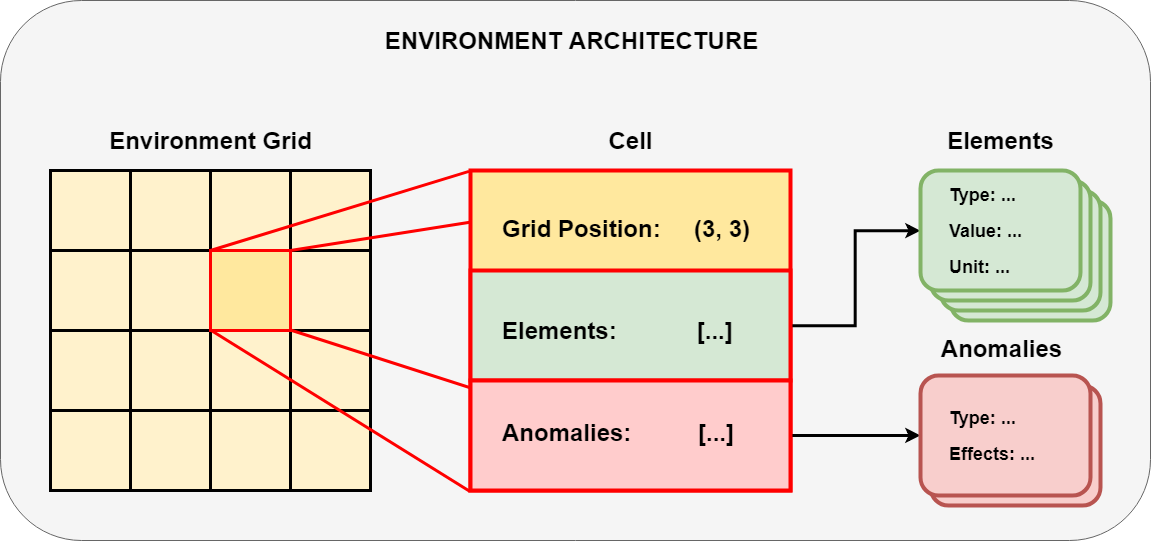
\includegraphics[width=1.0\columnwidth]{Figures/environment_model.png}
  \caption[Environment Data Architecture]{A visual model of SCOUt's \texttt{Environment} class architecture. An environment is made up of cells which hold information about the environment. This information includes any present element type or anomaly.}
  \label{fig:environment_model}
\end{figure}

The \texttt{Environment} class (Appendix~\ref{appendix:environment_class}) holds an $n \text{x} m$ 2D grid of uniformly sized $s \text{x} s$ square cells, where $n \text{x} m$ is the total area of the environment and $s \text{x} s$ is the area each cell represents within the environment.
A \texttt{Cell} (Appendix~\ref{appendix:cell_class}) holds $x$ and $y$ coordinates for its relative position within the \texttt{Environment}'s grid.
These coordinates do not reflect the actual size of the cell, only an index value for the order they appear within the 2-dimensional array data structure (e.g., see ``Position'' of ``Cell'' in figure~\ref{fig:environment_model}).
The environment's scale can easily be applied to the physical location of a cell as it is a shared global attribute within the \texttt{Environment} class.
If an element type or an anomaly is present within the area of the environment that the cell covers, it will be stored in an appropriate list within the \texttt{Cell} instance.

An element can be any measurable attribute within an environment.
For example, temperature, elevation and decibel levels are all attributes of the environment whose values can be measured.
All element types are all generalized by the abstract trait, \texttt{Element} (Appendix~\ref{appendix:elelment_trait}).
The trait has a set of attributes that an inheriting class must define to identify the element's type and how it behaves.
Each element type has \texttt{name} and \texttt{unit} attributes that are used for identification and denoting the unit of measurement.
The \texttt{value} attribute holds a numerical value for the measurement of each instance.
For example, an instance of the \texttt{Elevation} class (Appendix~\ref{appendix:elevation_class}) stores a measurement of the elevation level in feet for the area within a cell.
The \texttt{radial} flag, \texttt{lowerBound} and \texttt{upperBound} attributes guide and limit the values that can be set for each element type.
These are used when procedurally generating an environment (covered in section~\ref{sec:environment_builder}).

An anomaly is any object that may be of significance to an agent, such as a human or precious mineral.
Anomalies each have their own effects on element values in the environment around them.
Like \texttt{Element}, \texttt{Anomaly} and \texttt{Effect} (Appendix~\ref{appendix:anomaly_trait} and Appendix~\ref{appendix:effect_trait}) are both defined as a single trait that specific classes can inherit from.
An \texttt{Anomaly} class can occupy multiple cells, but must occupy at least one cell in an environment.
Anomalies can also have multiple effects on the values of different element types in its surrounding area.
Each \texttt{Effect} class defines a ``seed'' element and a range of the effect.
The \texttt{seed} attribute holds a specific instance of an \texttt{Element} class that will be present in the \texttt{Cell}s that the anomaly occupies.
The \texttt{range} then defines the radius of the area beyond the attribute's position that the effect will ``radiate.''
The term radiate is used because the effect will alter the element type's values in surrounding cells based upon how close they are to the source of the effect (the anomaly).

For example, \texttt{Human} (Appendix~\ref{appendix:human_class}) is an anomaly that takes the area of a single cell, and affects the temperature and decibel values in their environment.
If the human is much louder than the ambient noise level in the environment, there will be a sharp spike in decibel values in cells nearest the human, with a diminishing increase for values in surrounding cells.
Figure~\ref{fig:human_decibel_effect} shows a heatmap of decibel values in an environment that a human is present within.

\begin{figure}[!htb]
  \centering
  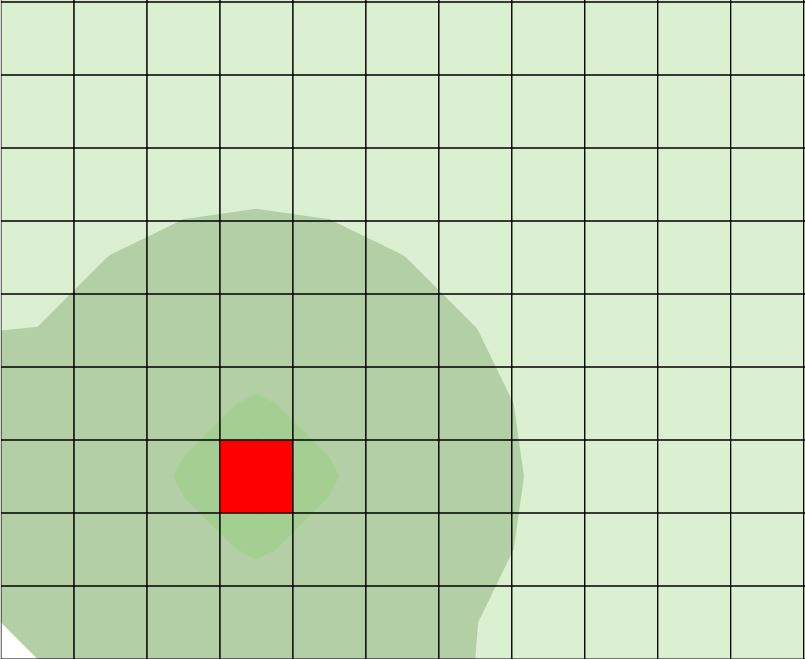
\includegraphics[width=0.6\columnwidth]{Figures/human_decibel_effect.JPG}
  \caption[Sound Effect Heatmap]{Heatmap of the layer of decibel values within an environment that contains a human. A darker shade of green represents higher values of decibel levels, lighter shades represent lower values, and the human's location is shown in red.}
  \label{fig:human_decibel_effect}
\end{figure}

One last important data structure is a \texttt{Layer} (Appendix~\ref{appendix:layer_class}).
A layer is designed in the same 2-dimensional structure as the \texttt{Environment} grid, but holds a collection of \texttt{Element} instances instead of cells (figure~\ref{fig:human_decibel_effect} is an example of a layer of decibel elements).
While layers are not direct members of the \texttt{Environment} class structure, they are crucial to building and analyzing the environment.
For this reason, instances of the \texttt{Layer} class are only generated on demand through method calls.


% ==============================================================================
% AGENT
% ==============================================================================
\section{Agents} \label{sec:agent}
Agents within this experiment are modeled based on a set of abilities that dictate how it will interact within an environment.
The \texttt{Agent} class defines these with state related attributes, physical limitations, a set of sensors that can be used, and a controller for decision making (Appendix~\ref{appendix:agent_class}).
The state related attributes of an \texttt{Agent} are health, energy level, an internal map, and its current position relative to the \texttt{Environment} grid.
Because SCOUt is focused on exploration-based operations, agent behaviors can be divided into two categories of actions: movement and scanning.
The agent can attempt to move one cell at a time in any of the four cardinal directions.
This allows the agent to reassess after each movement attempt.
Agents perform scanning actions to collect information about the immediate environment.
Any new information learned about the environment is stored in the agent's internal map.
The type of scanning actions that an agent can perform is based on the set of sensors the agent has equipped.
The agent's controller is in charge of analyzing the current state and deciding the next action to be performed.
To simulate the interactions that will occur between an agent and an environment, mobility and durability attributes are defined for each agent.
These will dictate how an agent can move within the environment and the types of effects each element type within the environment will have on the agent.
Figure~\ref{fig:agent_model} shows the internal agent architecture and how it applies to an external environment.

\begin{figure}[!htb]
  \centering
  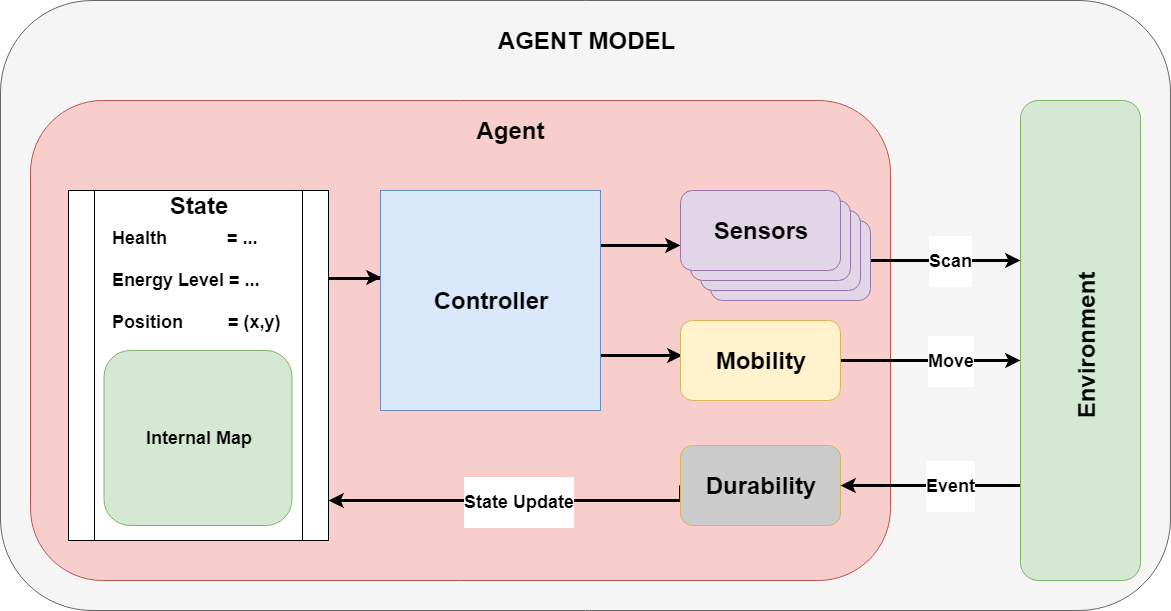
\includegraphics[width=1.0\columnwidth]{Figures/agent_model.png}
  \caption[Agent-Environment Interaction Diagram]{Visual model of the \texttt{Agent} class and how it interacts with an environment. A controller makes action decisions based on the agents current state. The agent will then attempt to perform the selected action within its environment. The agent's state will then be updated based on the resulting event.}
  \label{fig:agent_model}
\end{figure}


\subsection{Sensor} \label{subsec:sensor}
Sensors are defined using the same trait-class-instance architecture as \texttt{Element} and \texttt{Anomaly}.
The \texttt{Sensor} class (Appendix~\ref{appendix:sensor_class}) models a scientific instrument that could be used for gathering data measurements of a specific element type.
Each class defines the element type it is able to measure, the energy it costs to use, its effective range, and two flags indicating if the element type is hazardous or considered an indicator for the given operation.
When performing a scan, the sensor will sweep 360 degrees around the agents location and gather data within the circular area (figure~\ref{fig:sensor_range}).
The circular scan area is calculated with the sensors range as the radius and the agent's position as the center.
Any element values that were previously unknown to the agent are then added to the internal map.
Hazardous elements are flagged in a \texttt{Sensor} class instance when its element type has the potential to cause harm to the agent.
The indicator flag is set when the element type is believed to be an important data type related to the operation.
For example, if an agent was searching for a human, temperature and decibel sensors would be flagged as indicators since their values can potentially help lead the agent to the human.

\begin{figure}[!htb]
  \centering
  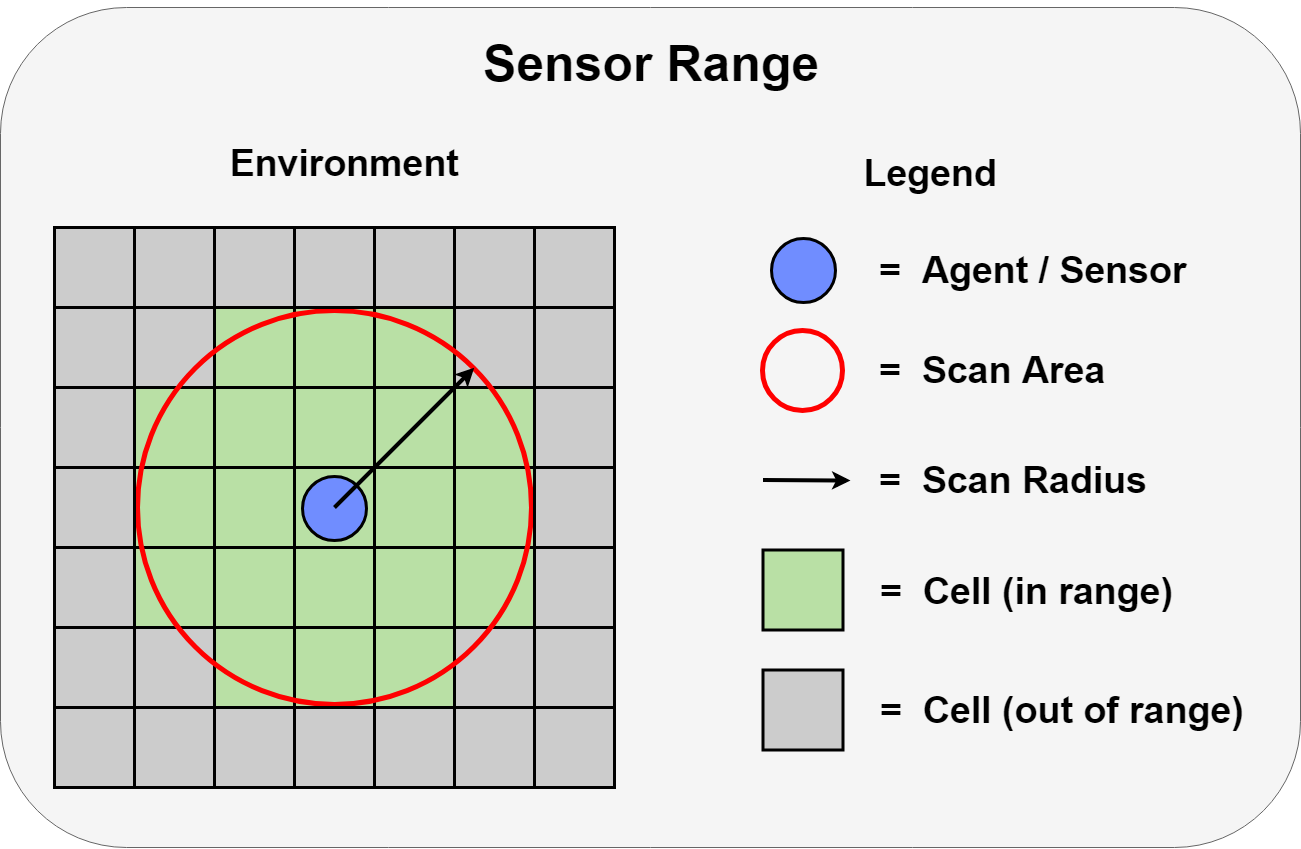
\includegraphics[width=0.70\columnwidth]{Figures/sensor_range.png}
  \caption[Sensor Scan Range Diagram]{Diagram of a sensor's effective range within a grid of environment cells. The sensor will collect present element values for cells in range. The type of values collected is dependent upon the element type that the sensor is designed for.}
  \label{fig:sensor_range}
\end{figure}


\subsection{Mobility} \label{subsec:mobility}
\texttt{Mobility} is a standalone class  that will determine the physical limitations of the agent when moving within an environment (Appendix~\ref{appendix:mobility_class}).
In real-world scenarios, agents often have to trade off functionality and mobility.
For example, if a drone was modeled as the agent, it would have a higher range of mobility, but would likely sacrifice the number of sensors that could be carried.
A wheeled robot loaded with multiple sensors would likely have decreased mobility but could collect a wider variety of data.
An agent's mobility is defined by the maximum slope an agent can climb, the minimum slope an agent can traverse before taking ``fall damage,'' a resistance factor, and the energy cost required for movement.
The resistance factor is used to scale the amount of fall damage that the agent may take.
Movement and slope costs are used to calculate how much energy is used when attempting a movement action.
The total amount of energy used is calculated based on the distance moved, and the slope of the elevation between the agent's current position and the position that it attempts to move to (equation~\ref{eq:movement_cost}).

\begin{capeq}[!htb]
  \begin{equation} \label{eq:movement_cost}
    energyCost = (1.0 + (slope * slopeCost)) * dist * movementCost
  \end{equation}
  \caption[Movement Energy Cost]{Equation to calculate the energy required for an agent to move within an environment. This is based on the agent's $movementCost$ and $slopeCost$, and the physical $slope$ and $distance$ that is traveled.}
\end{capeq}


\subsection{Durability} \label{subsec:durability}
Like many other data structures in this platform, \texttt{Durability} (Appendix~\ref{appendix:durability_class}) factors are defined per element type.
These factors model how an agent will be affected by different element types they come in contact with during an operation.
For example, consider an environment with pools of water in it.
Most robots would be damaged when emerged in water, but an amphibious robot's durability could be modeled such that it would be impervious to water damage.
Durability is defined by an upper and lower value threshold, and a resistance factor.
The thresholds define what values of an element type the agent can be exposed to before it begins to take damage.
The resistance factor between 0 and 1 (0 being no resistance and 1 being immune) then influences how much damage the agent will take when in contact with values beyond these thresholds (equation~\ref{eq:duribility_damage}).

\begin{capeq}[!htb]
  \begin{equation} \label{eq:duribility_damage}
    damage = |v - threshold| * (1.0 - resistance)
  \end{equation}
  \caption[Agent Damage]{Damage calculation based on an agent's $resistance$ to an element type with value $v$ that is above or below a durability $threshold$.}
\end{capeq}

\subsection{Actions} \label{subsec:actions}
Agents interact with an environment via movement or scanning actions.
These two categories cover the exploration and research aspects that are required for most surveillance operations.
The agent's controller is in charge of deciding what action to perform.
Figure~\ref{fig:agent_actions} shows an example of an agent within an environment considering both a movement and a scanning action, and the new states that would result from selecting either of them.

\begin{figure}[!htb]
  \centering
  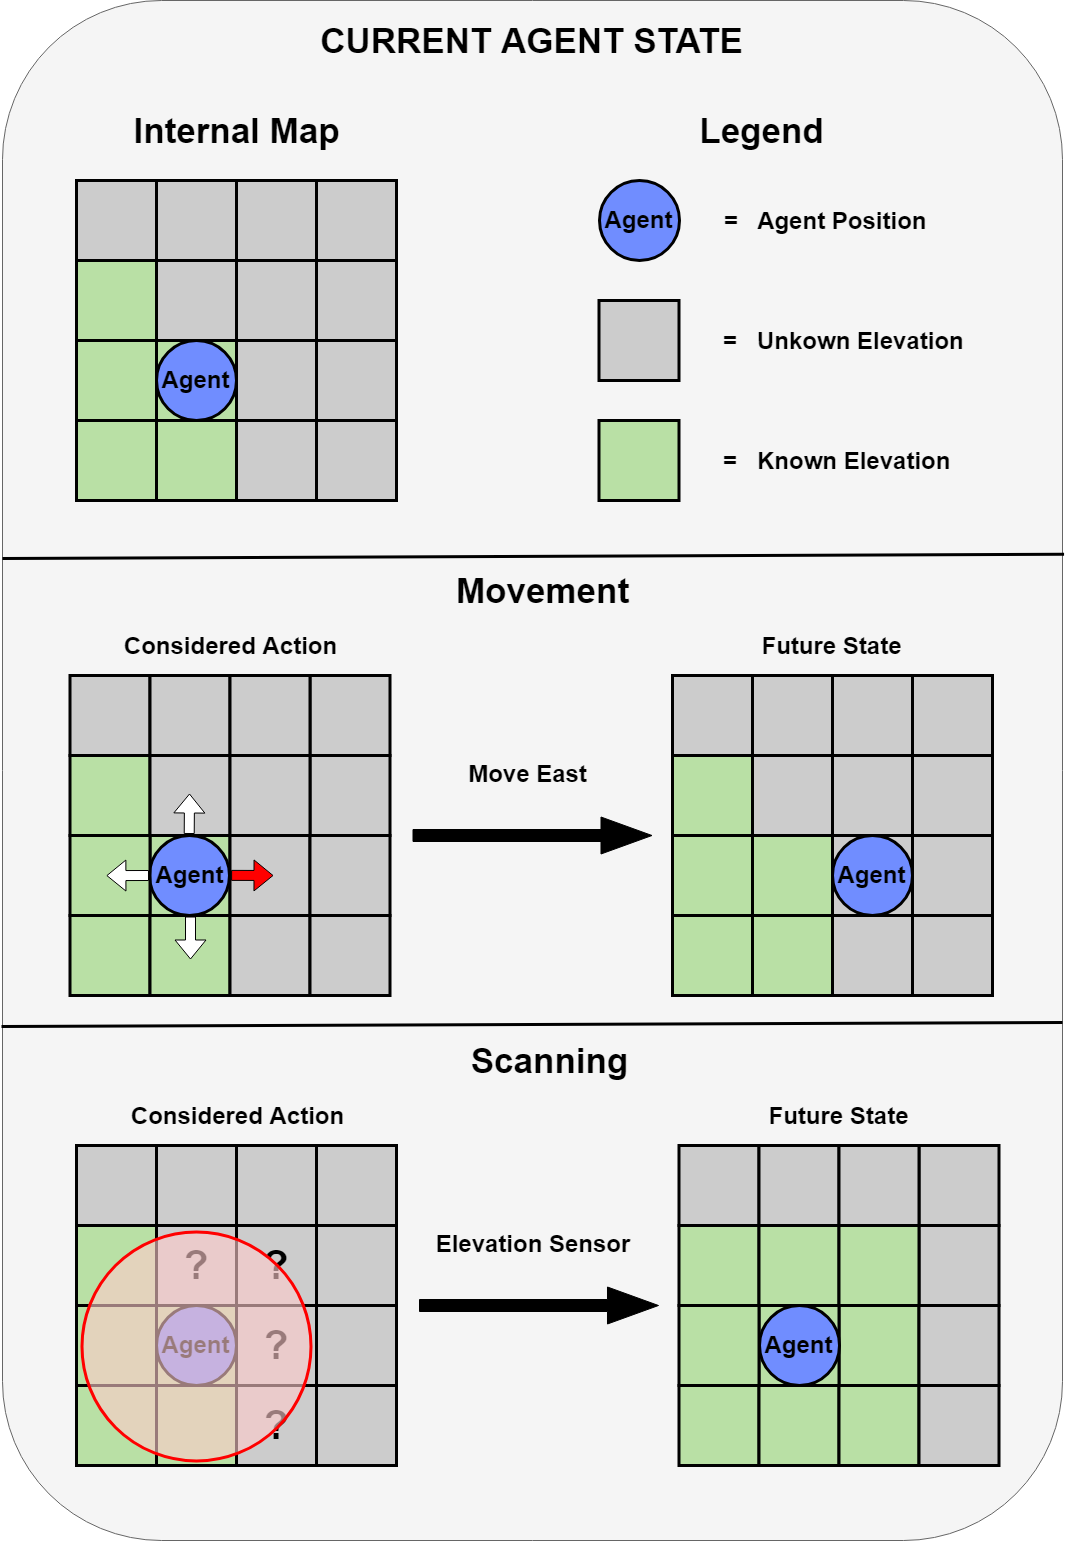
\includegraphics[width=0.8\columnwidth]{Figures/agent_actions.png}
  \caption[Agent Action Types]{Example of an agent considering a movement action and a scanning action, along with the resulting states caused by each of these actions.}
  \label{fig:agent_actions}
\end{figure}

In simulation, movement is handled by changing the agent's current position to an adjacent cell in one of four direction (``north,'' ``south,'' ``west,'' or ``east'') based on the orientation of the environment's grid of cells.
Moving a single cell at a time gives the agent the opportunity to reassess its current state before selecting the next action.
Distance covered by successful movement will inherently be equal to the size of the cells within the simulated environment.
Each time an agent attempts to move to a new cell, elevation levels will be compared between the current and new cell to check if movement is possible, or if it results in damage (based upon the agent's mobility).
After the action has been attempted, changes to health and energy level are calculated based upon the agent's durability factors.
If the movement action is successful, the current position is updated.

An Agent can also perform scans of the environment using equipped sensors.
For each cell that falls within the sensor's search radius, the value for the sensor's given element type is extracted.
These values are then added to the agent's internal map if they did not previously exist there.
Through repeated scanning, the agent will begin to fill its internal map with data collected from the surrounding environment.
Data collected in the internal map can then be used by the controller to determine what actions would be most beneficial to the goal at hand.


\subsection{State Representation} \label{subsec:state_representation}
For controllers to intelligently choose among actions, they need to have sufficient data about the agent and surrounding environment.
The agent's position, health and energy level can easily be analyzed, but the internal map containing the known environment is a very large data structure to analyze each time the controller must choose an action.
For this reason, the data structure is simplified to reduce memory usage and the computational effort required to analyze a state.
\texttt{AgentState} (Appendix~\ref{appendix:agentstate_class}) is a minimal data structure that contains all of the useful information necessary for a controller to make intelligent decisions.
Instead of a 2-dimensional array of cells, the internal map is represented as a list of \texttt{ElementState}s (Appendix~\ref{appendix:elementstate_class}), where each \texttt{ElementState} is a summary of the data known about a specific element type.

Element states contain useful information about what is currently known about a specific element type during an operation.
The indicator flag can cue the controller on whether the element type is being analyzed in order to progress the goal at hand.
If the goal was to map out the elevation levels in an environment, the elevation \texttt{ElementState} would be flagged true.
If the goal was to find a human, the temperature and decibel \texttt{ElementState}s would be marked true, as irregular changes in these values could indicate the presence of the human.
The hazard flag is used to mark any element that could potentially cause harm to the agent.
For example, the presence of water, large changes in elevation, and extreme temperatures could potentially cause damage and would be flagged as hazardous.
We also track the percent of known element values that are within range of the corresponding sensor.
Technical information of each \texttt{ElementState} is divided into four quadrants, where each quadrant has its own state.
Because agent movement is defined as north, south, west and east, we can collapse known information from the internal map into four quadrants (figure~\ref{fig:quadrants}).

\begin{figure}[!htb]
  \centering
  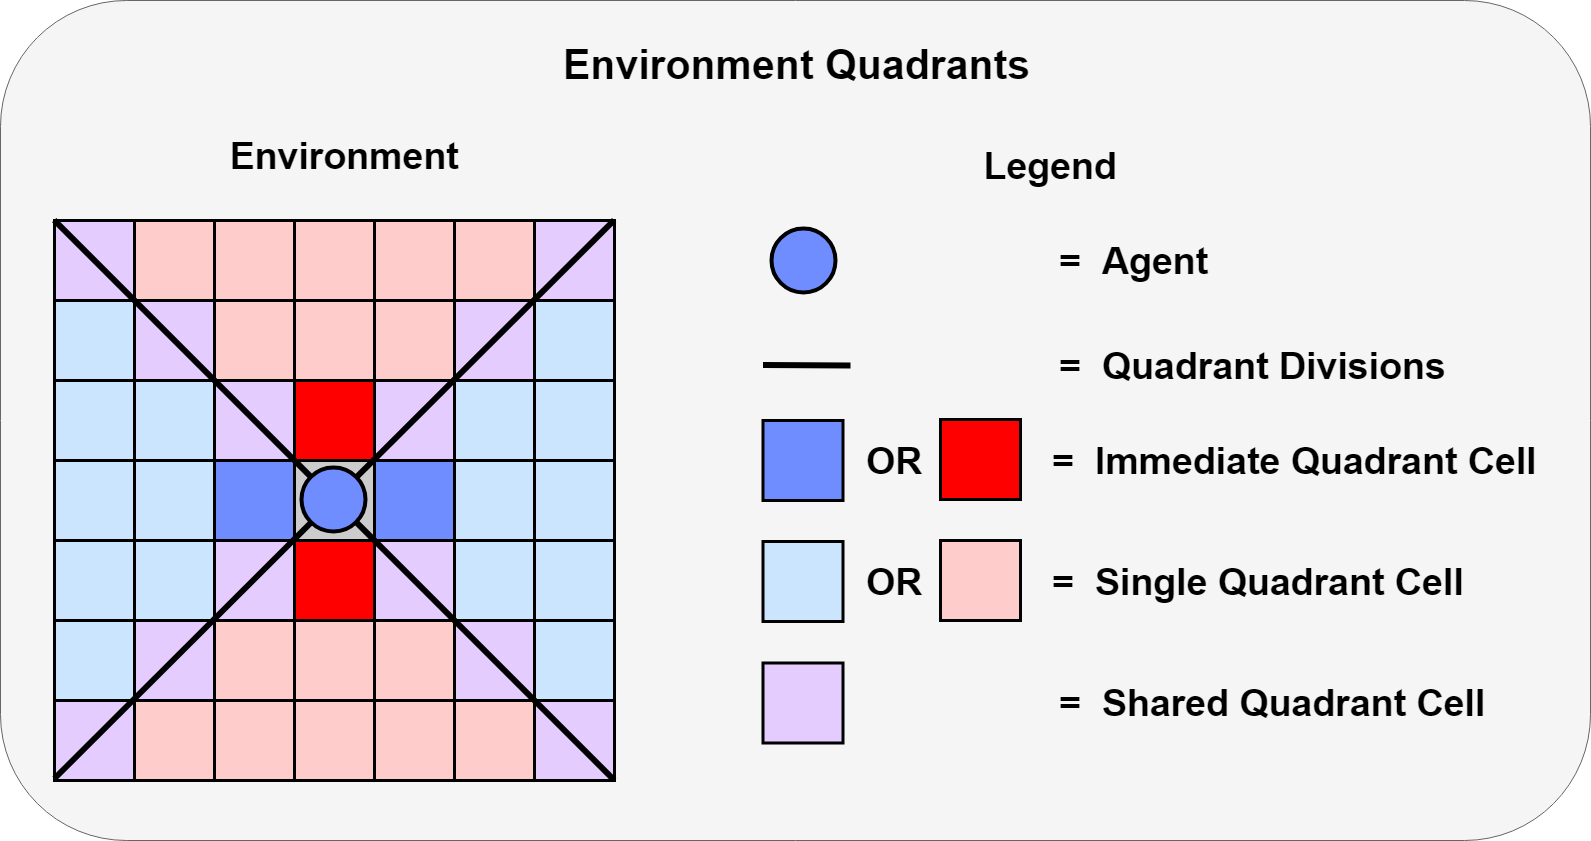
\includegraphics[width=1.0\columnwidth]{Figures/quadrants.png}
  \caption[Environment Quadrant Division]{Diagram showing how an environment is divided into quadrants relative to an agent's position within a grid of cells.}
  \label{fig:quadrants}
\end{figure}

Each quadrant is defined using a \texttt{QuadrantState} (Appendix~\ref{appendix:quadrantstate_class}).
To reflect the amount of information that is known about an element type within the quadrant, the \texttt{QuadrantState} first looks at the percentage of cells in the agent's internal map that hold known values.
If there are known values within the quadrant, the averages will be reflected in the \texttt{QuadrantState}.
Additionally, if the value in the cell immediately adjacent to the agent's current position is known, it will also be reflected in the \texttt{QuadrantState}.
Average and immediate values are stored as ``differentials'' relative to the value in the current cell.
Average differential takes the difference between the current cell's value and the average of all known values in the quadrant's collection of cells.
Immediate differential takes the difference between the current cell's value and the cell immediately adjacent to it.
In doing so, the controller will have data that is relative to the agent's current position.


\subsection{Controller} \label{subsec:controller}
A controller is the goal driven decision model that an agent will use when navigating within an environment.
The agent will pass its current state to the controller, along with a list of valid actions that it can execute.
The controller will then decide which action to take.
Controllers are defined as an extendable trait (Appendix~\ref{appendix:controller_trait}).
The \texttt{Controller} trait requires that inheriting classes define a \texttt{setup} and \texttt{shutdown} function to perform any initializations or final actions once an operation has ended, and a \texttt{selectAction} function.
The \texttt{selectAction} function is where the controller's decision model is implemented.
This function takes the list of valid action and the current \texttt{AgentState} as input, and returns a single action for the agent to perform.
Specific Controllers and their schemas are analyzed and discussed in chapter~\ref{ch:controllers}.




% ==============================================================================
% OPERATIONS
% ==============================================================================
\section{Operations} \label{sec:operations}
To explore the efficiency and adaptability of the intelligent controller, many different scenarios need to be simulated.
All simulations are made up of three main components: an agent, a goal, and the environment.
Different combinations of each component allow the creation of a large variety of scenarios.
Each simulation follows a defined process called an operation (figure~\ref{fig:operation}).
An operation will simulate an agent's attempt to complete a goal within an environment, record data for each event that occurs between the agent and environment, and the final outcome.
These data collections are denoted as short-term and long-term events respectively.

\noindent
Short-term events are collected each time the agent performs an action.
They include:

\begin{itemize}
  \setlength\itemsep{-12pt}
  \item The agent's state when the action was selected
  \item Any changes to the agent's internal state (health or energy reduction)
  \item \singlespace{If the action performed was successful (could it move, did it have enough energy to complete the action)}
  \setlength\itemsep{0pt}
  \item A short term reward for the outcome of the action
\end{itemize}

\noindent
A long-term event is only collected once at the simulated operation ends.
It includes:

\begin{itemize}
  \setlength\itemsep{-12pt}
  \item Status of internal variables (health and energy)
  \item Number of actions taken during operation
  \item Goal completion
  \item An overall long term reward
  \item Long term reward given to each action taken
\end{itemize}

\begin{figure}[!htb]
  \centering
  \includegraphics[width=1.0\columnwidth]{Figures/operation.png}
  \caption[Operation Diagram]{Diagram depicting the flow of an operation where an agent is attempting to complete a goal within an environment. The agent will continuously select actions to perform until the goal is successfully completed or it is no longer operational. An agent is no longer operational if its health or energy are depleted due to the events that occur as it interacts with the environment. Once an operation has completed, each action the agent attempted will receive a short-term and long-term score.}
  \label{fig:operation}
\end{figure}


\subsection{Goals} \label{subsec:goals}
Because SCOUt is designed for exploration, two goal types are analyzed: anomaly searching and element mapping.
This is not to say that SCOUt would be limited to operations which only involve these types of tasks.
SCOUt is intended to be \textit{integrated} with other tasks.
For example, if the entire task of a robot was to traverse a hazardous area to find a certain mineral for extraction.
SCOUt would be used to guide exploration in the environment and detect the mineral.
When the mineral is found, SCOUt's process would then be completed successfully, and a separate process could take over for the actual extraction, or the location could be recorded by SCOUt and another agent could be deployed.
After the other agent or process completes its task, SCOUt could continue to search for more deposits of the mineral or return to base.
For anomaly searching goals, the agent is required to find a specified anomaly within an environment.
This tests SCOUt's ability to use environmental clues to track down the anomaly.
For example, if the agent was looking for a human after a natural disaster, it could use data such as temperature and decibel readings to locate the person.
The element mapping goal is straitforward.
The agent must map out as much data about the specified element type as possible.


\subsection{Rewards} \label{subsec:rewards}
In addition to goal completion, an agent must also be observant of its health and energy throughout the operation.
The more efficiently an agent can complete an operation the better.
The overall performance of an agent is measured by both its ability to complete the task at hand, and the safety and efficiency of the actions taken.
These performance measurements are calculated on a short-term and long-term basis and come in the form of ``rewards.''

\subsubsection{Short-Term Rewards}
Short-term rewards are given each time an agent performs an action (algorithm~\ref{algorithmic:short_term_reward}).
Energy and health depletion are major factors in this reward.
If the action required an excessive amount of energy or resulted in damage to the agent, the reward is decreased.
Other factors that come into play depend on the specific action taken.
If the agent attempted to move to a new area and failed to move (e.g., a hill was too steep to climb) a deduction is made.
A small increase in reward is applied if the agent moves into an unexplored area.
If the agent uses a scanner, the reward is calculated to reflect the amount of new information learned.
This penalizes the agent from using a scanner multiple times in the same area, as it is not an efficient use of energy.

\begin{algorithm}
  \setstretch{1.2}
  \caption[Short-Term Reward Calculation]{Calculate the short-term reward for an event caused by an agent's action within an environment. $W_{item}$ denotes the attributed weight for $itemReward$.}
  \begin{algorithmic} \label{algorithmic:short_term_reward}
    \REQUIRE $W_{health} \in \left[0, \infty \right)$
    \REQUIRE $W_{energy} \in \left[0, \infty \right)$
    \REQUIRE $W_{action} \in \left[0, \infty \right)$
    \REQUIRE $maxHealth \leftarrow 1$
    \REQUIRE $maxEnergy \leftarrow 1$
    \REQUIRE $actionType \in \{movement, scanning\}$
    \REQUIRE $cellVisitedBefore \in \{true, false\}$
    \REQUIRE $scanDatas \in \left[0, \infty \right)$
    \REQUIRE $newScanDatas \in \left[0, scanDatas \right]$
    \REQUIRE $remainingHealth \in \left[0, 1 \right]$
    \REQUIRE $damageTaken \in \left[0, 1 \right]$
    \REQUIRE $energyUsed \in \left[0, 1 \right]$
    \ENSURE $shortTermScore \in \left[0, 1 \right]$
    \IF {$remainingHealth == 0$}
      \RETURN $shortTermScore \leftarrow 0$
    \ELSE
      \STATE $damageInverse \leftarrow (maxHealth - damageTaken) / maxHealth$
      \STATE $energyUseInverse \leftarrow (maxEnergy - energyUsed) / maxEnergy$
      \STATE $healthReward \leftarrow damageInverse \times W_{health}$
      \STATE $energyReward \leftarrow energyUseInverse \times W_{energy}$
      \IF {$actionType == movement$}
        \IF {$cellVisitedBefore == false$}
          \STATE $actionReward \leftarrow W_{action}$
        \ELSE
          \STATE $actionReward \leftarrow 0$
        \ENDIF
      \ELSE
        \STATE $actionReward \leftarrow (newScanDatas / scanDatas) \times W_{action}$
      \ENDIF
      \STATE $rewardsTotal \leftarrow healthReward + energyReward + actionReward$
      \STATE $W_{total} \leftarrow W_{health} + W_{energy} + W_{action}$
      \RETURN $shortTermScore \leftarrow rewardsTotal / W_{total}$
    \ENDIF
  \end{algorithmic}
\end{algorithm}


\subsubsection{Long-Term Rewards}
Long-term rewards are calculated once an operation is over using algorithm~\ref{algorithmic:long_term_reward}.
Operations end when the agent has successfully completed its goal or has depleted its health or energy.
To reflect these scenarios, reward is determined by the goal completion, remaining health, and remaining energy.
Even if a goal is completed, the agent could receive a low score if it was ``reckless'' and took lots of damage or used large amounts of energy.
The long-term reward is then propagated backwards through all the actions that were taken.
The actions performed immediately before the end of the operation are given highest score.
Previous actions then receive diminishing reward based on equation~\ref{eq:longtermscore_distribution}.

\begin{algorithm}
  \setstretch{1.35}
  \caption[Long-Term Reward Calculation]{Calculate the long-term reward for an agent's performance in an operation. $W_{item}$ denotes the attributed weight for $itemReward$.}
  \begin{algorithmic} \label{algorithmic:long_term_reward}
    \REQUIRE $W_{goal} \in \left[0, \infty \right)$
    \REQUIRE $W_{health} \in \left[0, \infty \right)$
    \REQUIRE $W_{energy} \in \left[0, \infty \right)$
    \REQUIRE $goalCompletion \in \left[0, 1 \right]$
    \REQUIRE $remainingHealth \in \left[0, 1 \right]$
    \REQUIRE $remainingEnergy \in \left[0, 1 \right]$
    \ENSURE $longTermScore \in \left[0, 1 \right]$
    \STATE $gReward \leftarrow goalCompletion \times W_{goal}$
    \STATE $hReward \leftarrow remainingHealth \times W_{health}$
    \STATE $eReward \leftarrow remainingEnergy \times W_{energy}$
    \STATE $rewardsTotal \leftarrow gReward + hReward + eReward$
    \STATE $W_{total} \leftarrow W_{goal} + W_{health} + W_{energy}$
    \RETURN $longTermReward \leftarrow rewardsTotal / W_{total}$
  \end{algorithmic}
\end{algorithm}

\begin{capeq}[!htb]
  \begin{equation} \label{eq:longtermscore_distribution}
    actionLongTermReward(i) = longTermReward * {0.9}^{\frac{i*10}{n}}
  \end{equation}
  \caption[Action Long-Term Reward Attribution]{Equation representing the diminishing long-term reward that each of the $n$ actions will be assigned based on the $longTermReward$ the agent received for completing an operation, where $i$ is the current action's index within the operation event log.}
\end{capeq}


% ==============================================================================
% ENVIRONMENT GENERATION
% ==============================================================================
\section{Environment Builder} \label{sec:environment_builder}
The SCOUt \texttt{EnvironmentBuilder} is a tool for creating diverse environment models.
The tool is highly abstracted so that more details can easily be added to the model as needed while still maintaining a defined build process.
Environments are procedurally generated based upon a collection of parameters called an environment template.
These templates require minimal input to build unique environments.
An environment can be tweaked or even built entirely by hand, but the procedural generation process removes this overhead.
Procedural generation process:

\begin{enumerate}
  \setlength\itemsep{-12pt}
  \item Environment Template is given
  \item	Builder initializes a grid of empty cells
  \item	\texttt{ElementSeed}s are used to populate each present element type into the gird of cells
  \item	\texttt{TerrainModification}s are applied to manipulate their related element(s)
  \item	Anomalies are placed randomly within the environment
  \item	Anomaly effect(s) are applied to corresponding element(s) in neighboring cells
\end{enumerate}

% \todo{diagram}
% \todo{example seed}
% \todo{example environment}

\subsection{Environment Templates} \label{subsec:environment_templates}
Each \texttt{EnvironmentTemplate} (Appendix~\ref{appendix:environmenttemplate_class}) will act as a guide in the creation of an instance of the \texttt{Environment} class.
A template can create similar, but unique environments each time it is used by the \texttt{EnvironmentBuilder}.
This allows testing and training agent controllers multiple times in similar conditions, while still providing a dynamic range of scenarios that the agent may face in each generated environment.
Each template is comprised of the name, dimensions and scale of the environment along with lists of \texttt{ElementSeed}s, \texttt{TerrainModification}s and anomalies to be applied.


\subsection{Element Seeds} \label{subsec:element_seeds}
The environment builder begins by procedurally generating one layer of elements at a time.
Each \texttt{Element} class has a companion class called an \texttt{ElementSeed} which holds parameters used to produce a layer of its element type, and a unique function defining how procedural generation will take place to produce the layer.
The generation of each layer is modeled on how the element type's values may vary in a real-world scenario.
Parameters within each Seed are set to default values that can also be overridden by creating a new instance of the \texttt{ElementSeed} (Appendix~\ref{appendix:elementseed_trait}).
This can change how the values within the layer will vary.


The environment builder will use each \texttt{ElementSeed} to produce each layer of elements.
Resulting layers will be temporarily stored in a list until the end of the build process so they can easily be manipulated before being stored into corresponding cells within the \texttt{Environment} grid.
Some layers are easier to generate than others.
Latitude and Longitude layers can be generated by calculating the distance each cell is from the origin point on the \texttt{Environment} grid).
For an example, let’s look at the \texttt{ElementSeed} for producing the elevation layer.

\begin{lstfloat}
  \caption[ElevationSeed Class]{Definition of \texttt{ElevationSeed} which extends the \texttt{ElementSeed} trait (\ref{appendix:elementseed_trait}). This provides the values and functions used to initialize a layer of elevation values in an environment.}
  \lstinputlisting{Codes/ElevationSeed.scala}
  \label{code:elevation_seed}
\end{lstfloat}

% \texttt{ElevationSeed} is a helper class which assists in the procedural generation of \texttt{Elevation} class instances within an environment. The seed has average and deviation values that guide its \texttt{buildLayer} function. These values are set to default values that can be overridden when an instance of this class is defined. The \texttt{buildLayer} function will begin by initializing an empty layer and then fill the layer with instances of the \texttt{Elevation} class. Each instance's value is determined by the \texttt{randomDeviation} function which returns a random value between the range of $\left[mean - deviation, mean +deviation\right]$.

The \texttt{ElevationSeed}’s \texttt{buildLayer} algorithm first initializes an empty \texttt{Layer}.
Next, it sets each (x,y) coordinate in the layer to an a random elevation value within a standard deviation of the average value provided [(average - deviation), (average + deviation)].
Once every Cartesian position has been set to an instance of elevation, the layer is then smoothed.
Smoothing is a function defined within the \texttt{Layer} class that will reduce strong variations of element values within the layer.
For elevation, this would equate to transforming a highly rigid surface into a smoother, more natural surface.

% \todo{smoothing pseudo-code}
% \todo{smoothing before-after photo}


\subsection{Terrain Modifications} \label{subsec:terrain_modifications}
Terrain modifications influence the basic landscape of the environment.
After each \texttt{ElementSeed} has produced a layer for the environment, \texttt{TerrainModification}s are applied one after another, taking care not to overlap modifications (e.g., we wouldn't want a hill to overlap with a valley and cancel each other out).
Each modification represents a severe alteration of one or more element type layers within the environment.
Following a similar process laid out by Doran and Parberry~\cite{doran_controlled_2010}, desired alterations are incorporated into the environment while allowing unique variations of each to develop.
Their controlled procedural generation process is used to produce landmasses that potentially have bodies and channels of water.
SCOUt's environment builder generalizes this process and extends it to allow multitudes of element types to be modified.
The \texttt{TerrainModification} trait provides an extendable template from which all types of modifications that can be applied (Appendix~\ref{appendix:terrainmodification_trait}).


\noindent
For an example, lets look at elevation again.

\begin{algorithm}
  \setstretch{1.1}
  \caption[Elevation Terrain Modification]{Algorithm for applying a terrain modification to a layer of elevation values denoted as cells. Note that the \texttt{Layer} is a collection of \texttt{Elevation} objects, not \texttt{Cell}s. However, it is easier to think of each location in the layer's grid as a cell, and is therefore denoted as such. The algorithm begins by initializes a random, unmodified cell. Next, it will modify neighboring cells until it has modified the requested \texttt{coverage} area or there are no unmodified, neighboring cells remaining. Once the modification process is completed, a smoothing function will be applied to cells in the modified area and cells in the surrounding area to ``blend'' the modified area into the rest of the environment (this prevents a plateau effect). The number of cells outside of the modified area that are smoothed is determined by the modification's \texttt{coverage} and \texttt{slope} set.}
  \begin{algorithmic} \label{algorithmic:terrain_modification}
    \REQUIRE $layer \leftarrow Array\left[Array\left[Elevation\right]\right]$
    \REQUIRE $modification \in \mathbb{Z}$
    \REQUIRE $deviation \in \mathbb{Z}$
    \REQUIRE $coverage \in \left[0,1\right]$
    \REQUIRE $slope \in \left[0,1\right]$
    \STATE $startCell \leftarrow layer.getRandomUnmodifiedCell$
    \IF {$\exists startCell$}
      \STATE $startCell.value \leftarrow modification$
      \FOR {$coverage \times layer.numCells$}
        \STATE $nextCell \leftarrow layer.getRandomUnmodifiedNeighbor$
        \IF {$\exists nextCell$}
          \STATE $mod \leftarrow \left[modification-deviation,modification+deviation\right]$
          \STATE $nextCell \leftarrow nextCell.currentValue + mod$
        \ELSE
          \STATE \textbf{BREAK}
        \ENDIF
      \ENDFOR
      \STATE $slopeRadius \leftarrow coverage / slope$
      \FOR {$modCell \in modifiedCells$}
        \FOR {$cell \in layer$}
          \STATE $dist \leftarrow distance(startCell, cell)$
          \IF {$dist \leq slopeRadius$}
            \STATE $layer.smooth(cell.x, cell.y, 2, dist)$
          \ENDIF
        \ENDFOR
      \ENDFOR
      \RETURN $layer_{modified}$
    \ELSE
      \RETURN $layer_{unmodified}$
    \ENDIF
  \end{algorithmic}
\end{algorithm}


Here we have an \texttt{ElevationModification} that will allow us to create hills and valleys within the environment.
Again following the approach of~\cite{doran_controlled_2010}, random, unmodified (x,y) positions are selected from the layer to begin with and updates their value to the specified modification value.
The modifier then performs ``walks'' to random, unmodified neighboring cells, updating their values within a standard deviation of the specified modification value.
These walks continue until the specified coverage area has been modified, or until there are no neighboring cells that can be modified.
A special layer smoothing algorithm is then applied to the elevation values in the modified area, as well as the immediate surrounding unmodified area to reduce rigidity and give a more natural change in values between neighboring cells.
This type of smoothing applies a given slopping factor within the modified area, allowing the \texttt{ElevationModification} to generate gentle hills or valleys or sharp cliffs depending on the slope defined.


\subsection{Anomaly Placement} \label{subsec:anomaly_placement}
Once all \texttt{TerrainModification}s have been applied, anomalies are placed into the environment.
Each specified anomaly is randomly placed into cell(s) in the \texttt{Environment}.
For anomalies that occupy more than one cell, neighboring cells are chosen at random until the \texttt{Anomaly}'s coverage area is met, or there are no neighboring cells that can contain the \texttt{Anomaly}.
The anomaly type is appended to each occupied cell's anomalies list for reference within the simulation.
After an anomaly has been placed, each of the anomaly's effects are applied.
An effect will alter the element values for the occupied and surrounding cells in the effected area.
These alterations are typically applied as a ``radiation.''
For example, a \texttt{Human Anomaly} might radiate heat and sound.
% To account for this, the radiation function is applied to the temperature and decibel values of cells in the effected radius.

Now that all \texttt{ElementSeed}s, \texttt{TerrainModification}s and \texttt{Anomaly} placements have occurred, the resulting layers containing their respective elements are populated into their corresponding (x,y) cell location within the \texttt{Environment} grid.
The resulting instance of an \texttt{Environment} class is then returned by the builder to the requesting party.



% ==============================================================================
% VISUALIZATION TOOL
% ==============================================================================
\section{Visualization Tool} \label{sec:visualization_tool}
The environment build tool provides a Graphical User Interface (GUI) for creating and visualizing environments.
Electron~\cite{electron} is used to render a web page contained within a standalone desktop application.
This allows the front end to be written in JavaScript, HTML and CSS and handle communication to the back end via HTTP over a localhost network.
A Scala library named http4s~\cite{http4s} is used to create a server on a localhost network for handling the HTTP requests from the front end.
Launching the GUI starts up the Scala server in a new terminal and opens the Electron window which will begin attempts to establish communication with the server.


\subsection{Home Page} \label{subsec:home_page}
Once a connection between the server and GUI has been established, the user is brought to the home page (figure~\ref{fig:visualizer_home_page}), where they can choose to generate a random environment, build a custom environment, load in an environment, or view an operation.
For a random environment, the user inputs the name and size of the environment and all other variables are set by the server.
Building a custom environment steps the user through a series of form pages to create an \texttt{EnvironmentTemplate}.
Loading an environment allows the user to select a saved environment or a saved template.
Selecting an operation will load the environment and log of all actions taken by an agent during a specific operation run that is saved in memory.
Once an environment has been generated and/or loaded by the server, it is returned to the GUI to be displayed.
The environment build tool will parse the returned environment into a graphical data representation, with interactive capabilities to explore the specific variables within the environment.
In the case that the user selected an operation, the user will additionally be able to step through the event log of an Operation.

\begin{figure}[!htb]
  \centering
  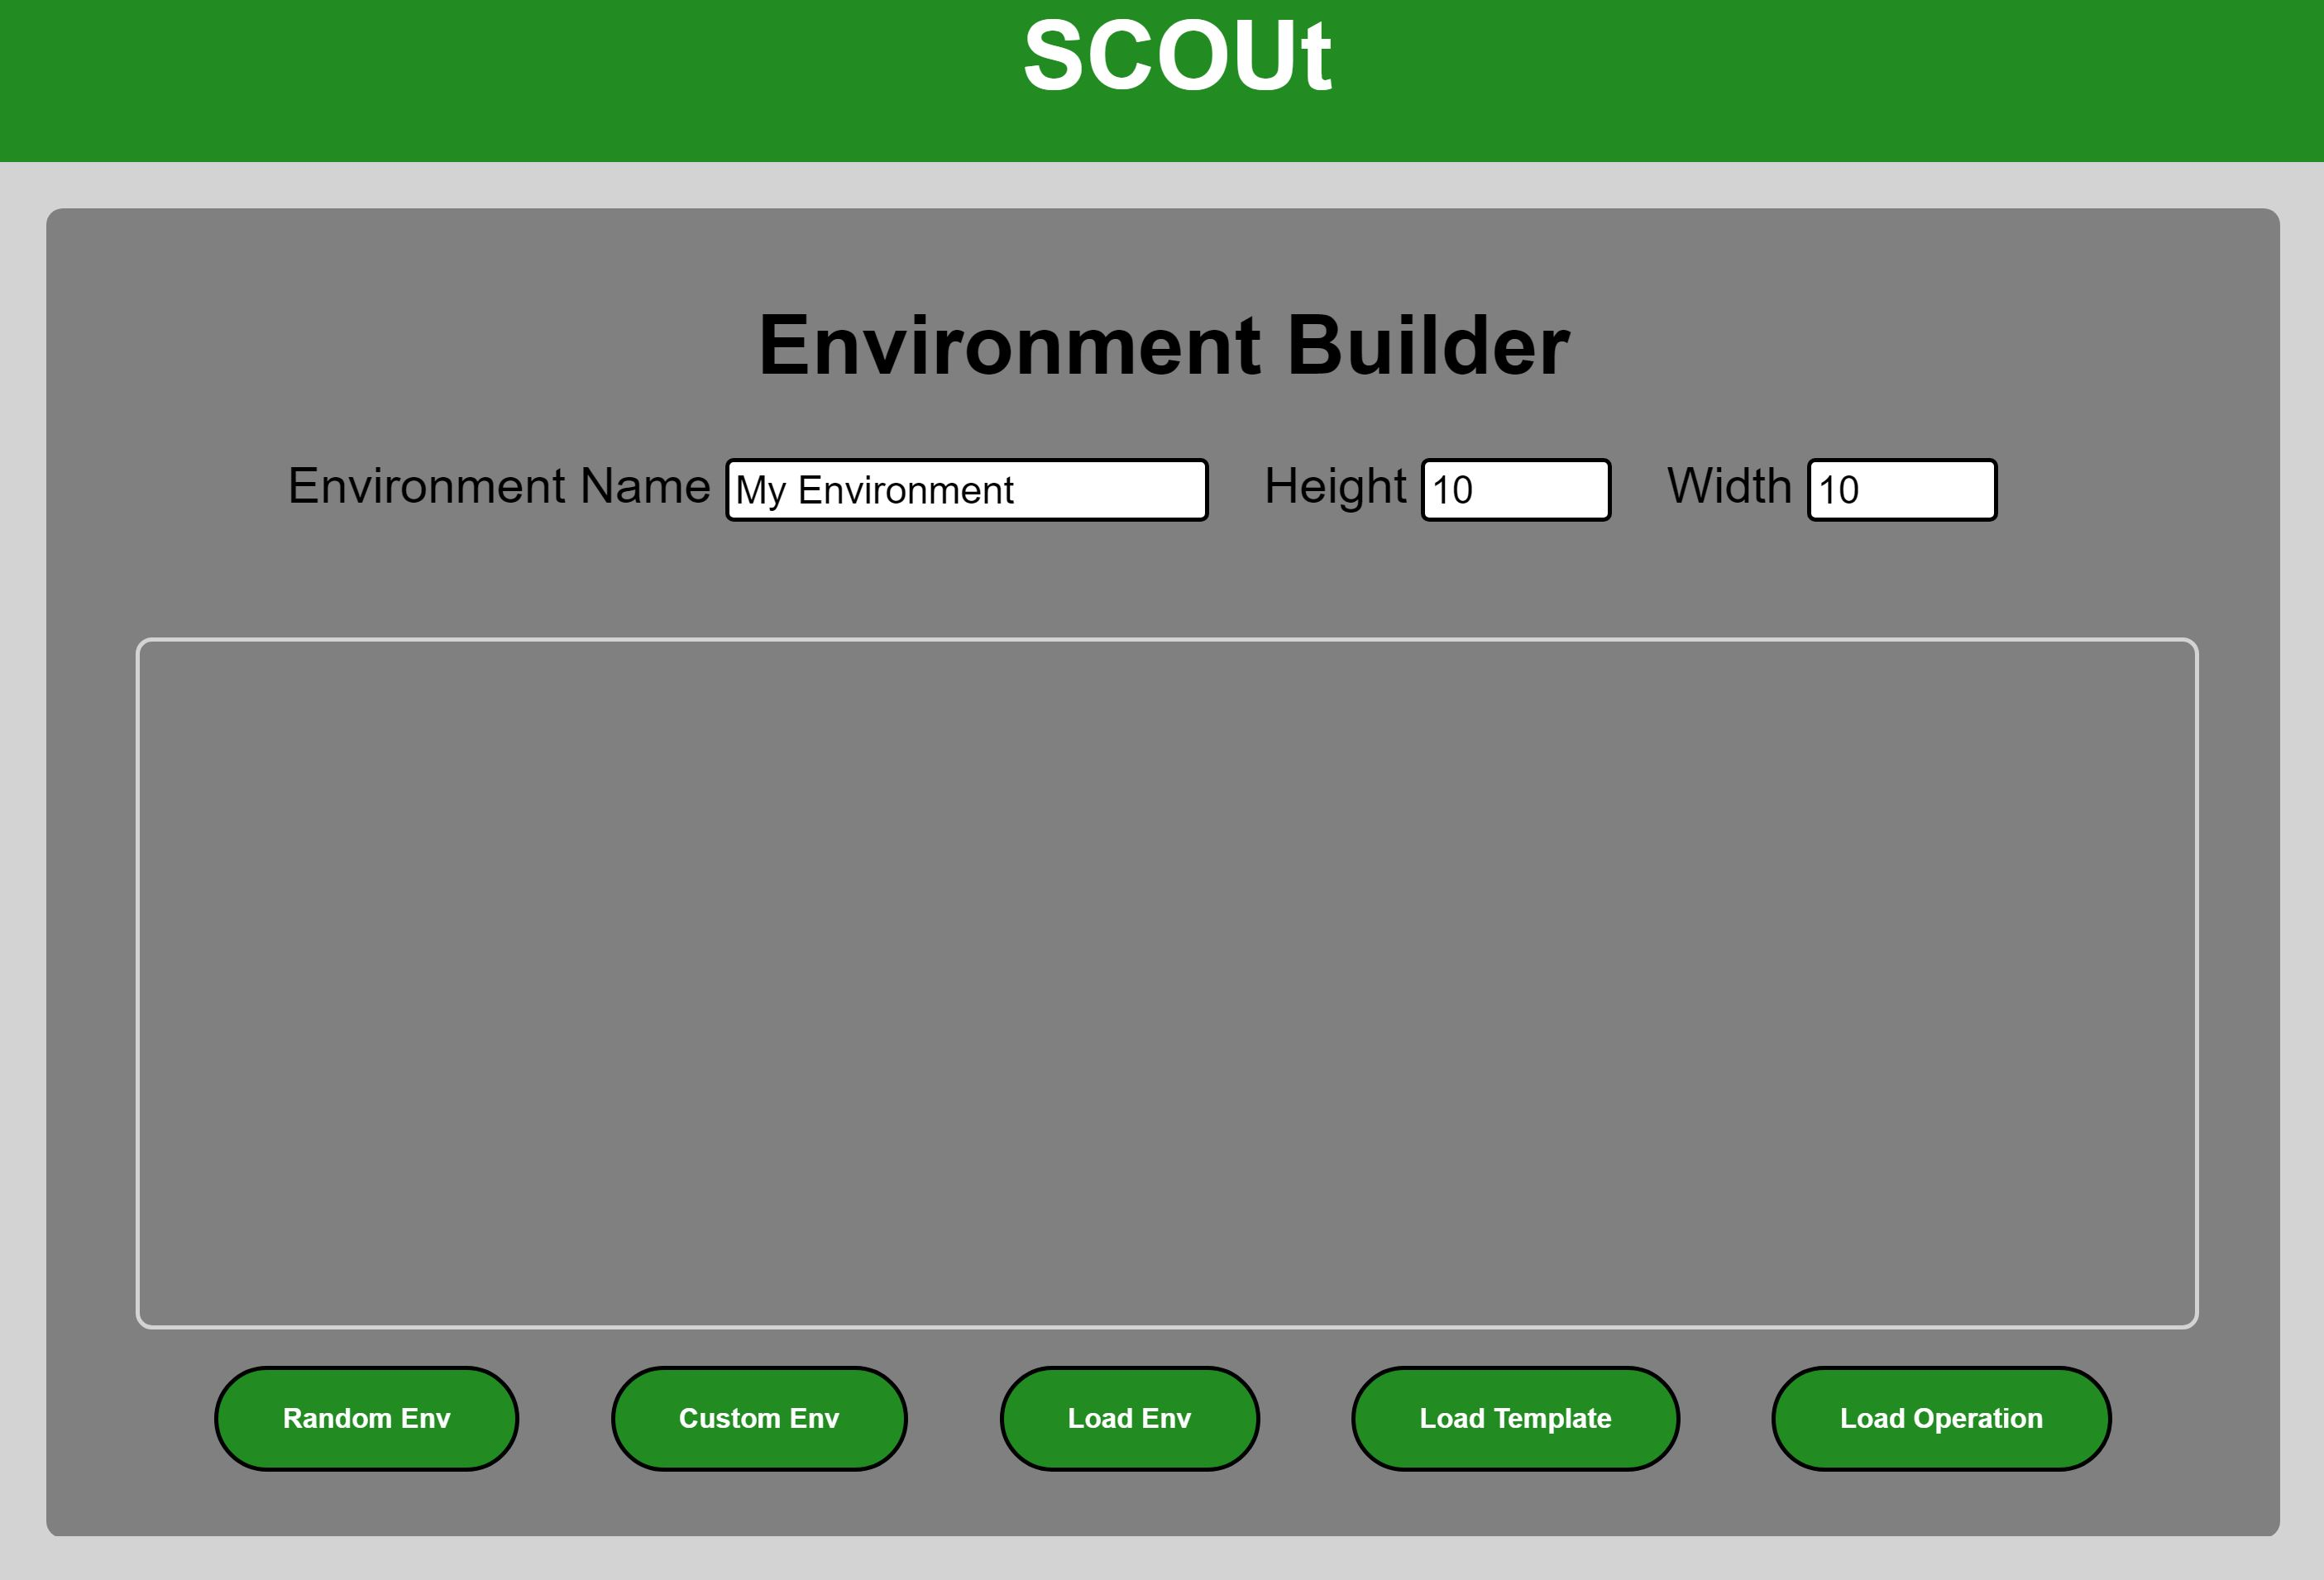
\includegraphics[width=1.0\columnwidth]{Figures/Visualizer/home_page.JPG}
  \caption[GUI Home Page]{Home page for SCOUt's graphical user interface. From here the user can select to generate a random environment, define a new environment template for generating an environment, load in existing environment or templates, or load an operation log to view the environment used in the operation and events that occurred.}
  \label{fig:visualizer_home_page}
\end{figure}

\subsection{Template Forms Page} \label{subsec:template_forms_page}
To create a template, the user will be presented with a series of forms with parameter input fields.
The forms are generated based on the available \texttt{Element}, \texttt{TerrainModification} and \texttt{Anomaly} classes that are defined in SCOUt's back end.
The first three forms will ask the user which element types, terrain modification and anomaly types they would like to include (e.g., figure~\ref{fig:example_form_page}).
Some elements such as elevation, latitude, and longitude, are required in all environments.
Once the user selects which features will be present in the environment templates, more forms will be generated for defining element seed data, anomaly seed data, and terrain modification parameter (e.g., figure~\ref{fig:example_form_page2}).
Each form within this process will save the user’s input data on the front end.
This allows the user to go back and edit form data while moving through the different form pages, as well as return and edit the form data after an environment has already been generated and loaded into the visualization page.
Form data is also set within required bounds and checked before submission.
Once the user has filled out all required form info, they can review their entire form entry from a single page and then submit it.
When submitted, the front-end data is converted into JSON data and sent in a request to the SCOUt server via a JavaScript fetch request.
An \texttt{Environment} instance is then built on the back end using the template parameters provided and returned to the front end where it is loaded into the visualization page.
Figure~\ref{fig:example_form_page} shows an example of an environment template form page, and figure~\ref{fig:forms_overview} shows an overview of the form input process.

\begin{figure}[!htb]
  \centering
  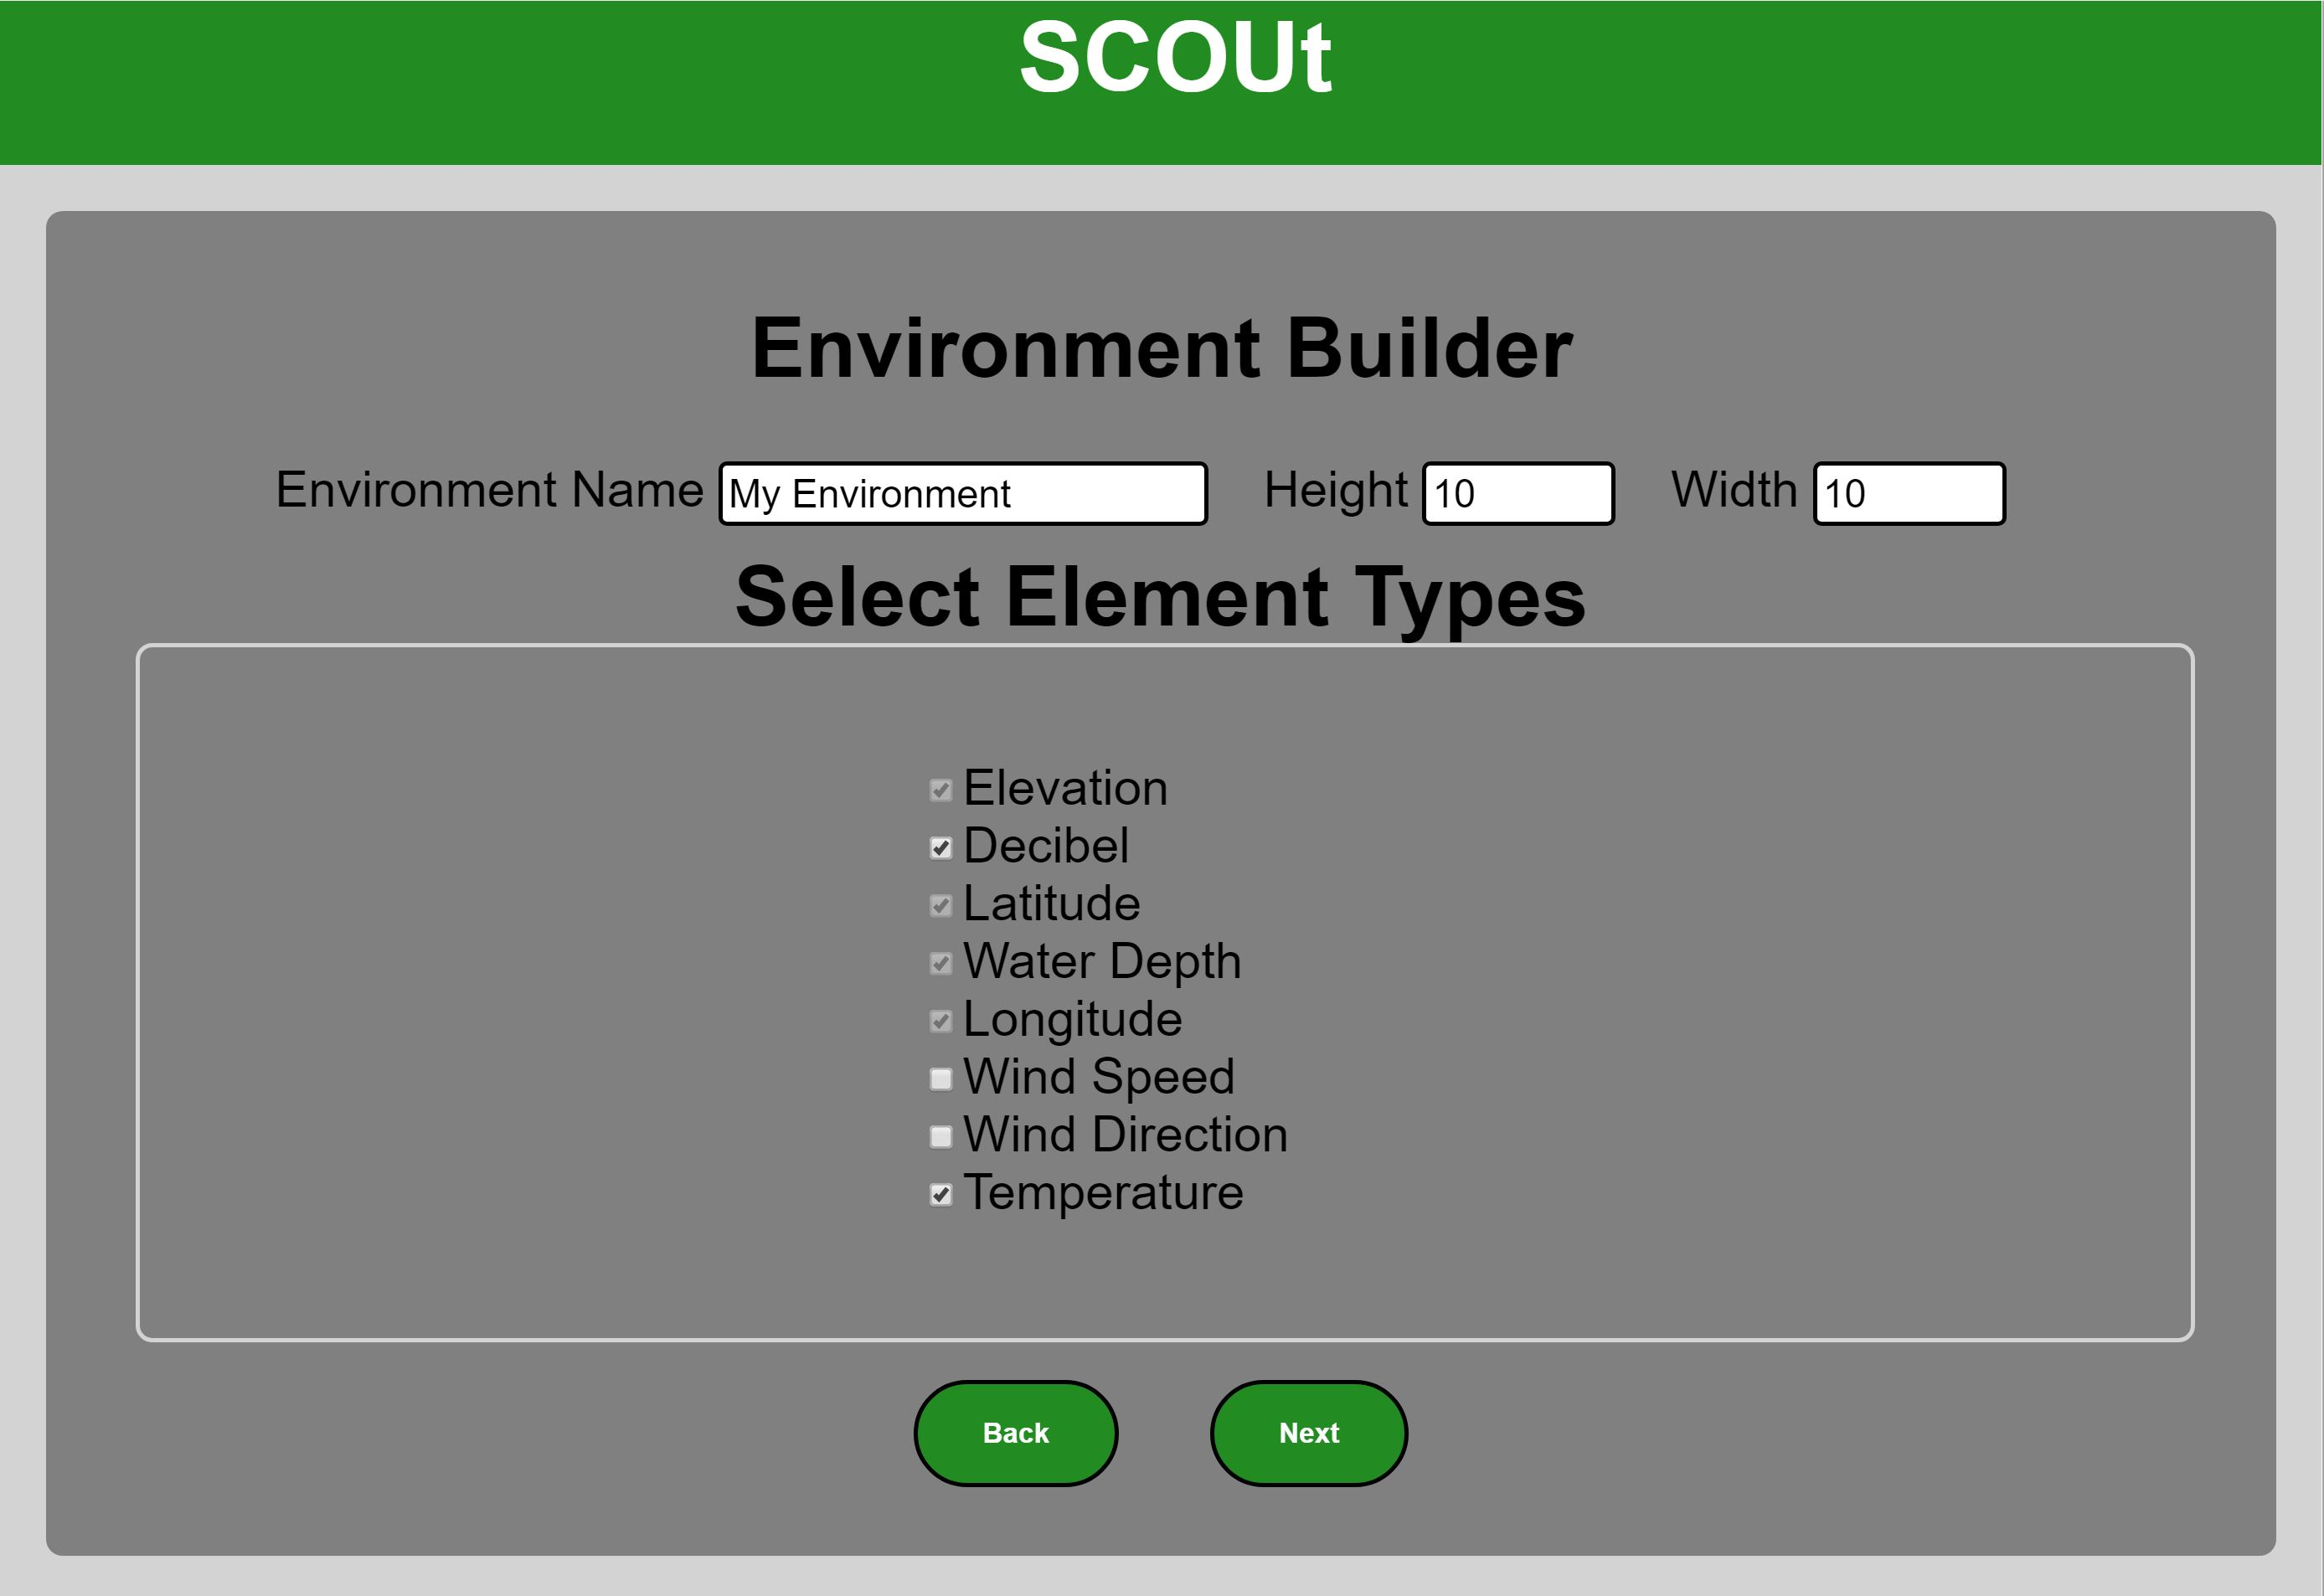
\includegraphics[width=1.0\columnwidth]{Figures/Visualizer/Forms/Visualizer-Forms-Element-Types.JPG}
  \caption[GUI Element Types Form]{User-input form page for selecting element types that will be present in an environment template. For each element type selected a new form page will be generated for the user to define seed data to guide how the element type will be procedurally generated into an environment.}
  \label{fig:example_form_page}
\end{figure}

\begin{figure}[!htb]
  \centering
  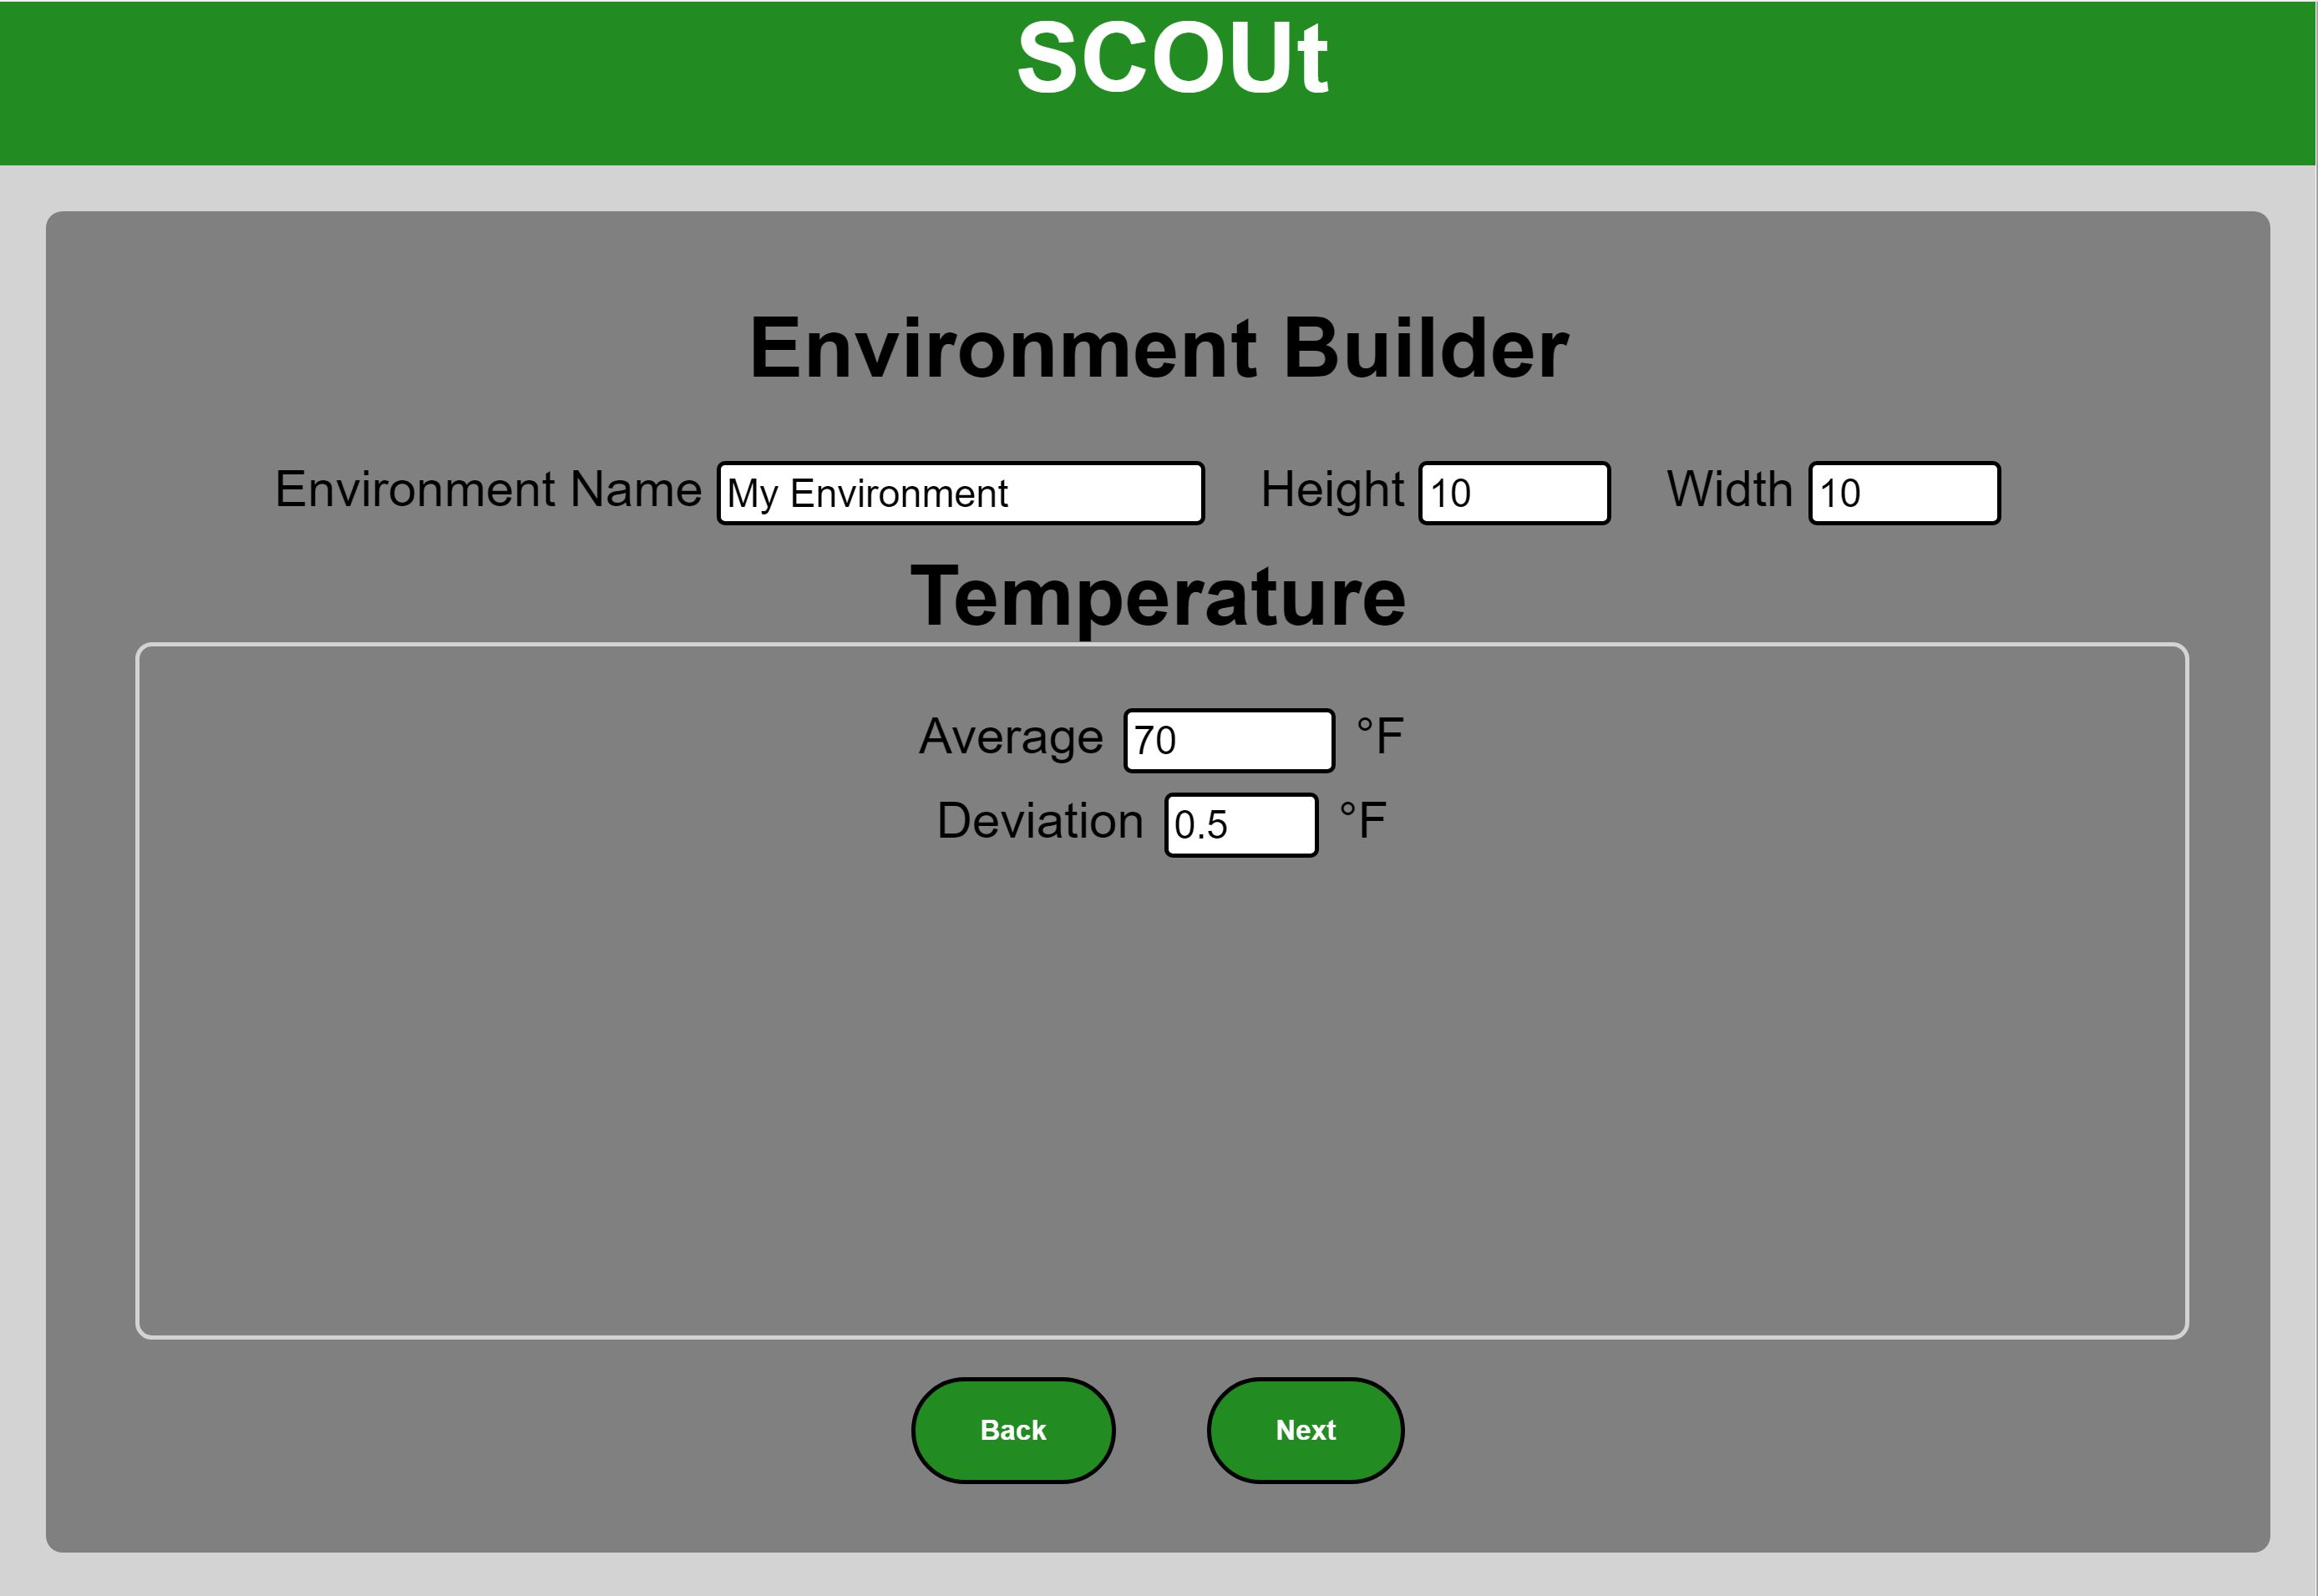
\includegraphics[width=1.0\columnwidth]{Figures/Visualizer/Forms/Visualizer-Forms-ElementSeed-Temperature.JPG}
  \caption[GUI Element Seed Form]{User-input form page for specifying element seed data for the ``Temperature'' element type. This seed data will be used in an environment template to procedurally generate an environment with an average ambient temperature of 70 degrees Fahrenheit and a standard deviation of 0.5 degrees from the average throughout the environment.}
  \label{fig:example_form_page2}
\end{figure}

\begin{figure}[!htb]
  \centering
  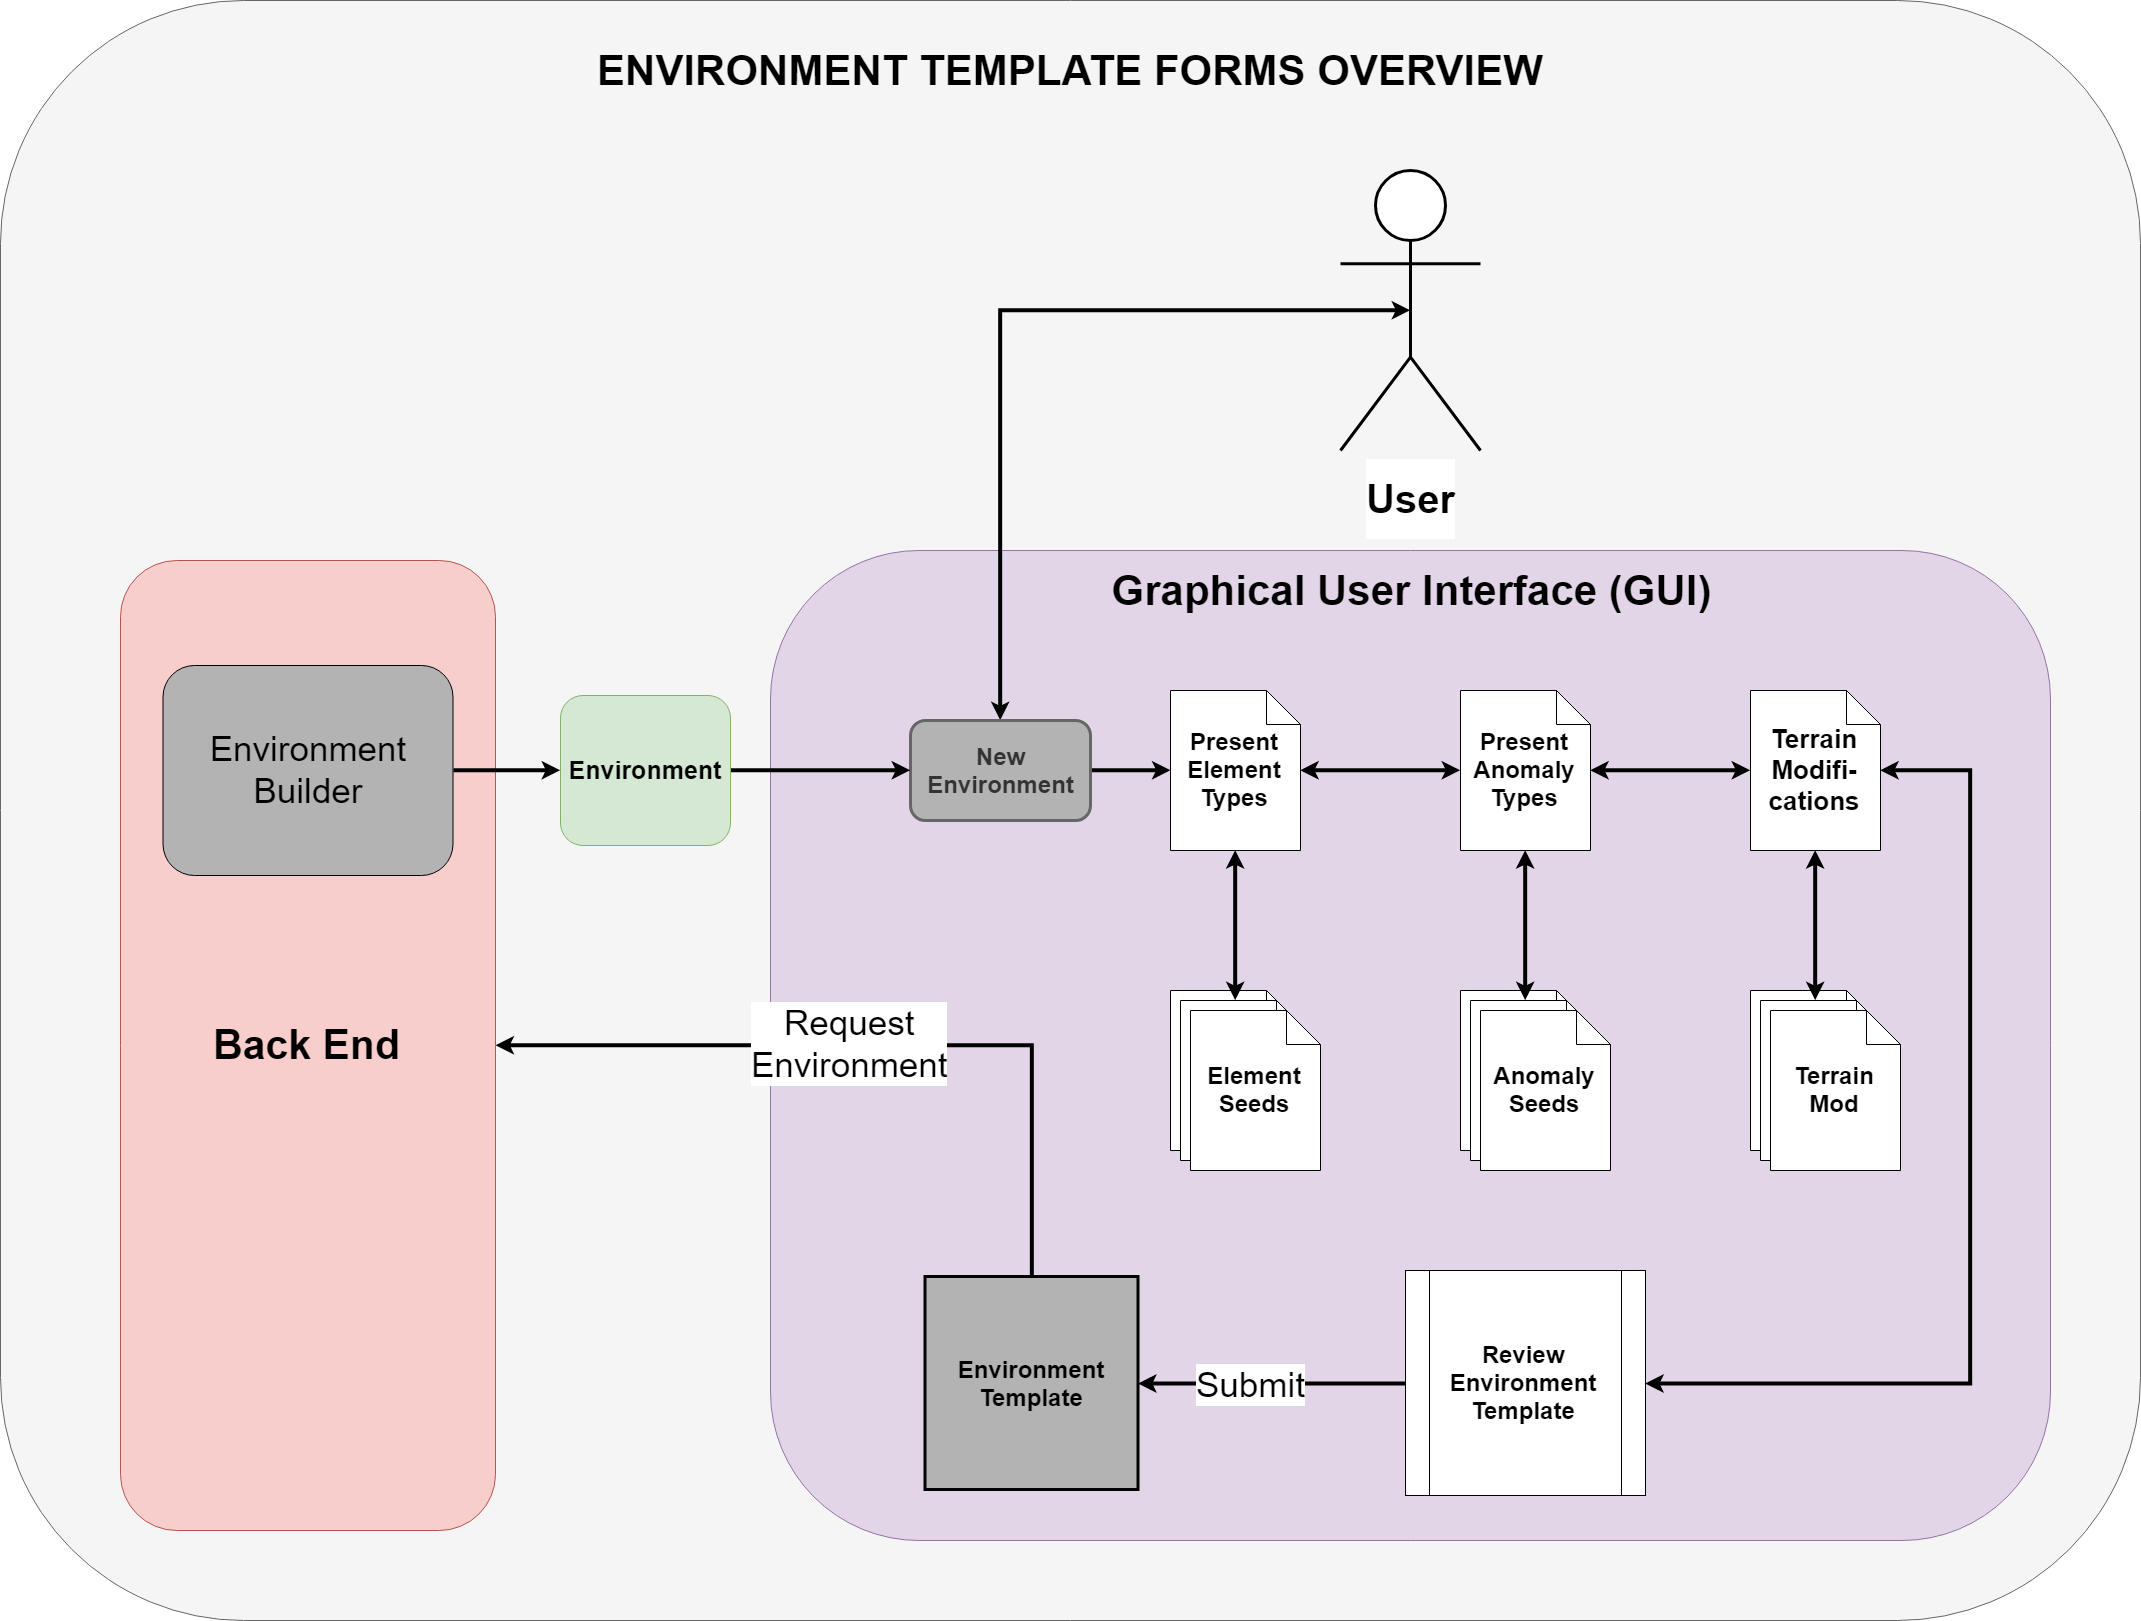
\includegraphics[width=1.0\columnwidth]{Figures/forms_overview.png}
  \caption[Environment Template Form Overview]{Visual overview of the form process that a user will complete to generate an environment. As the presence of element types, anomalies, and terrain modifications are selected, more forms will be generated for each of one. Once the user has filled out all the generated forms and has submitted them, an environment template will be created and sent to the back end. Here, the \texttt{EnvironmentBuilder} will create an instance of an environment based on the user's input and return it to the front end.}
  \label{fig:forms_overview}
\end{figure}


\subsection{Visualization Page} \label{subsec:visualization_page}
The visualization page provides an interactive overview of any given environment.
The main focus is on the display section where the entire environment grid is represented using heatmaps.
Different element layers can be viewed independently, anomaly locations can be highlighted, and specific element type values of a single cell can be viewed.
A main menu is also present to allow a user to perform higher level actions.
All of these interactive features are controlled by action, toggle and radio buttons within different sections of the visualization page.
The primary use of the visualization page is for creating environment templates and for debugging.
Debugging usage ranges from analyzing an environment that was used for testing an agent-controller setup or new features.
Examples of new features would be adding new classes (e.g., a new element type), or altering the process in which environments are generated and stored on the back end.

\begin{figure}[!htb]
  \centering
  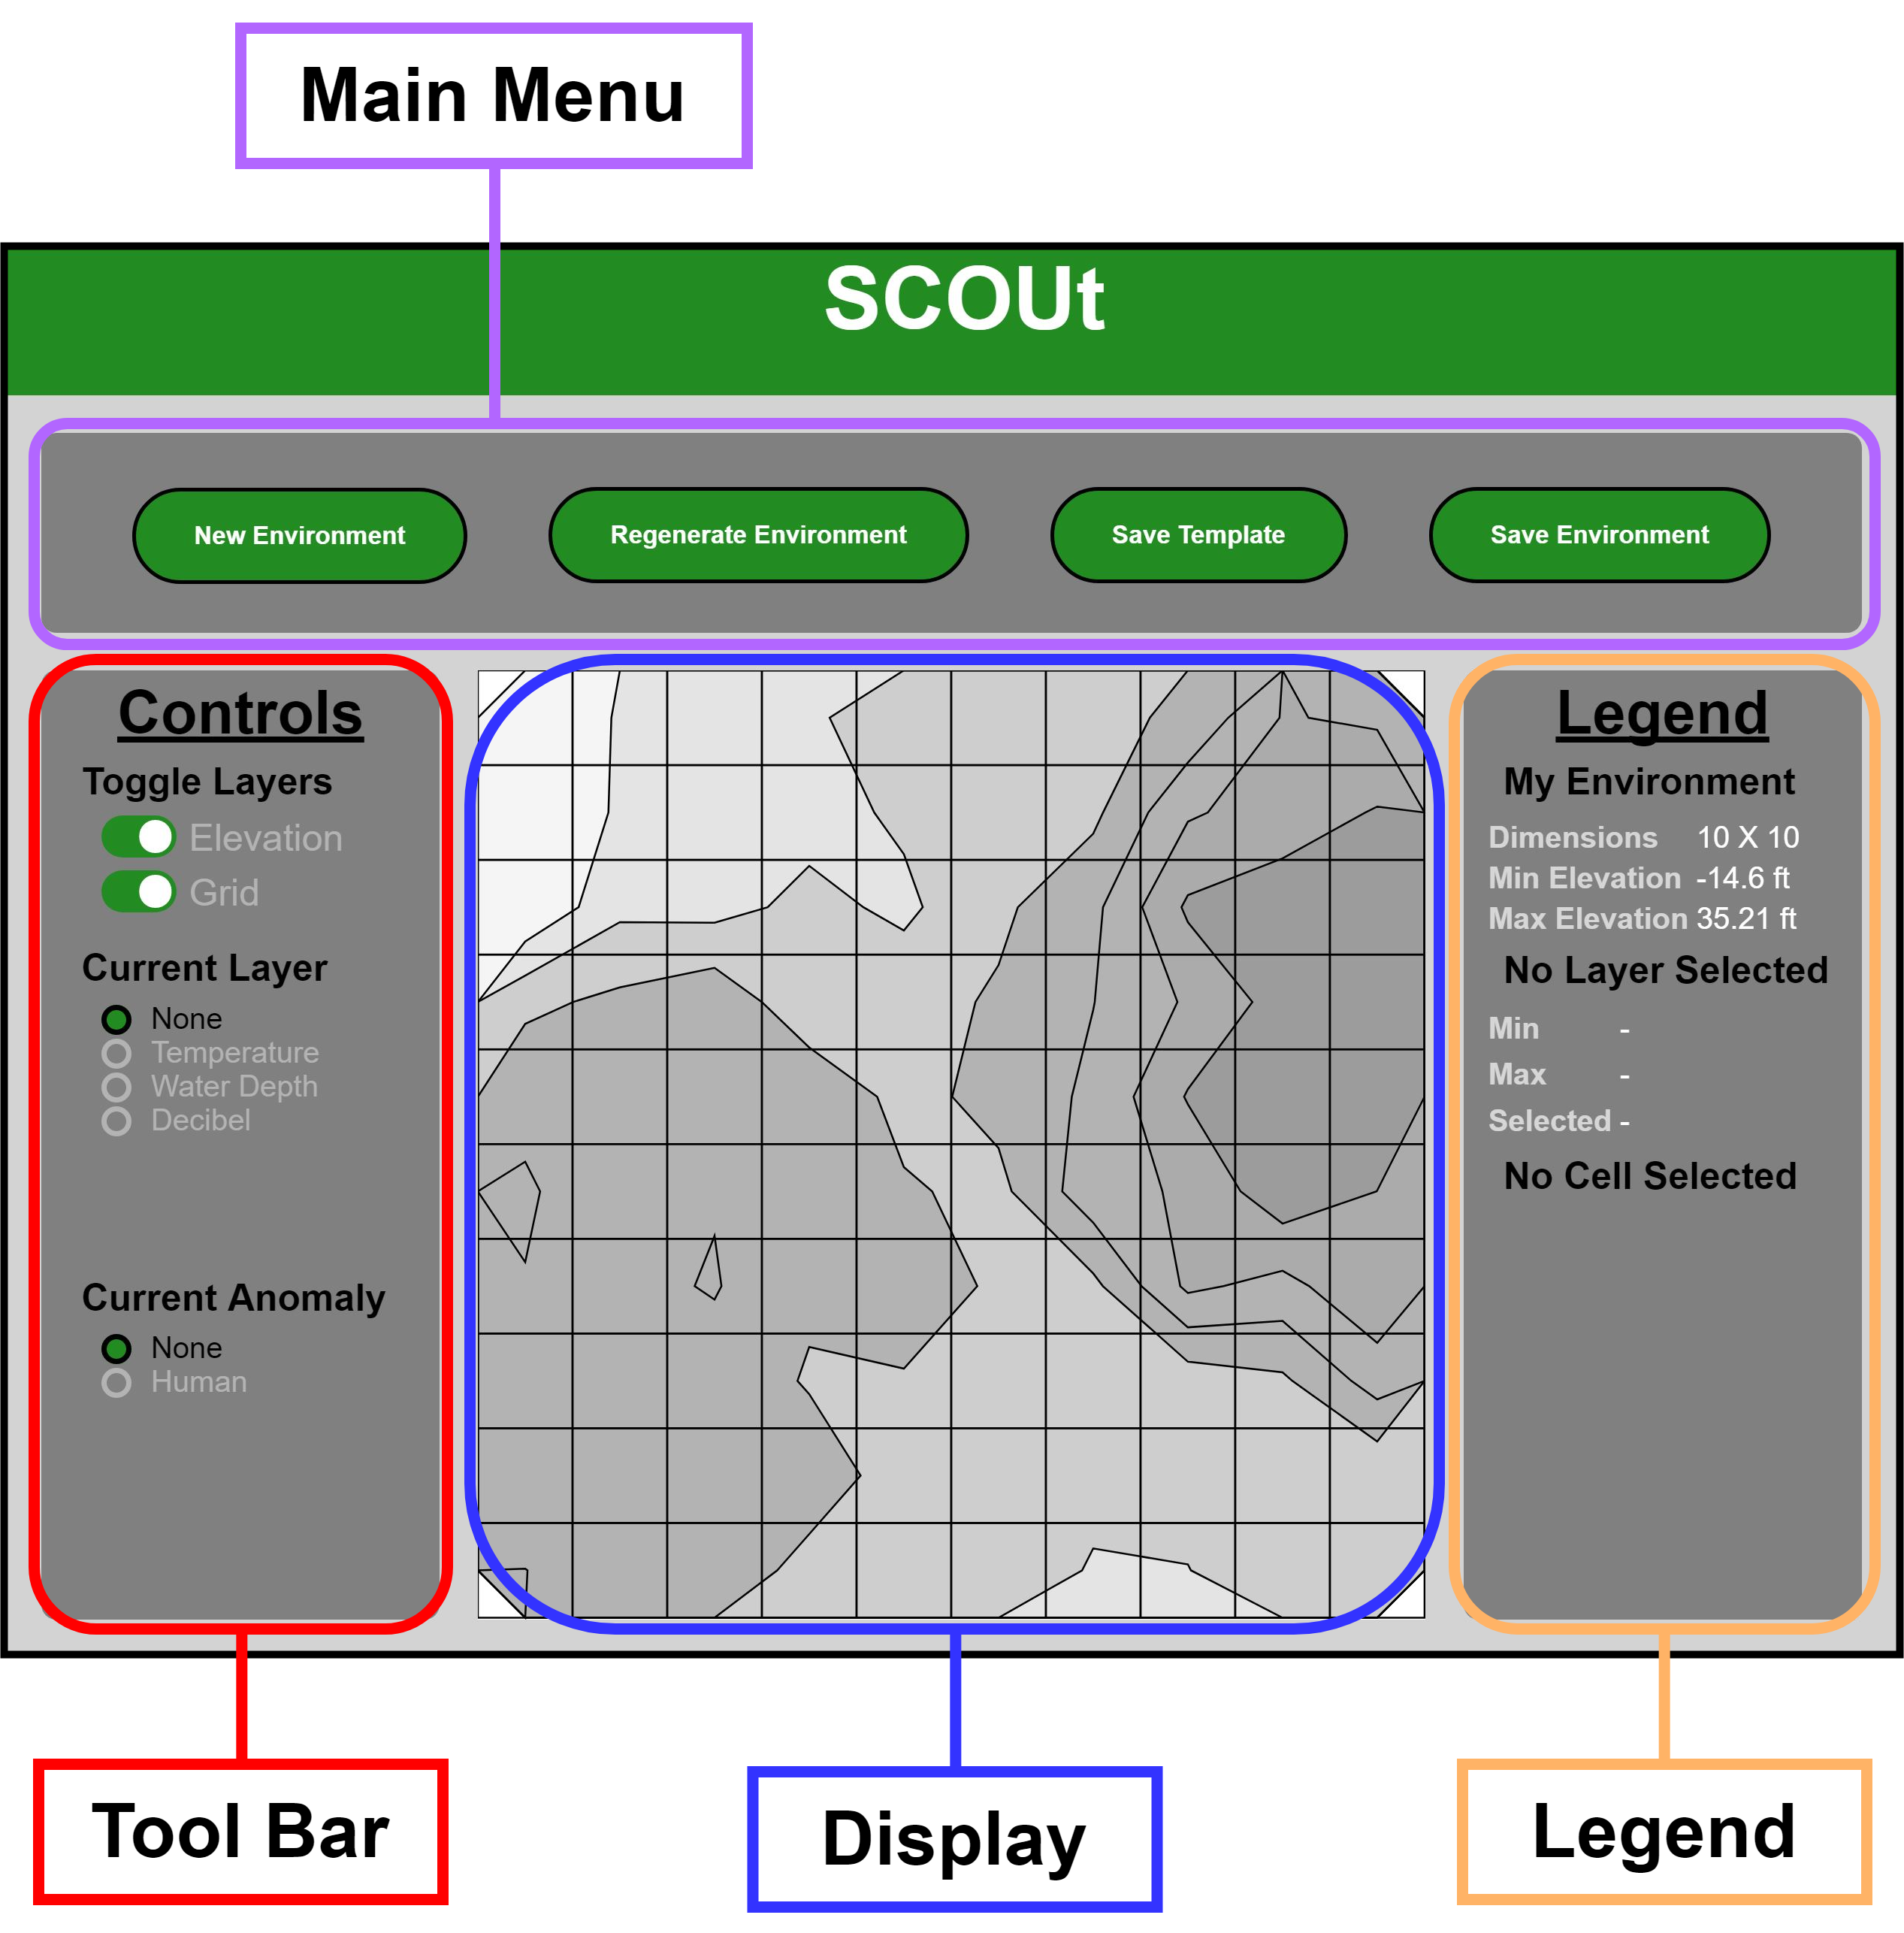
\includegraphics[width=1.0\columnwidth]{Figures/visualization_page.png}
  \caption[GUI Visualization Page]{Labeled view of the interactive environment-visualization tool with an example environment loaded. Each section of the page either displays information about the environment viewed or allows the user to interact with the view. The main menu also provides features to leave this view (via ``New Environment'').}
  \label{fig:visualization_page}
\end{figure}


\subsubsection{Main Menu}
The main menu provides high level functions to perform while using the environment build tool.
The main menu options are displayed at the top of the visualizer as a series of buttons.
The user can select buttons to return to the home page, regenerate or save the current \texttt{EnvironmentTemplate} (if an environment template is being used), or save the current \texttt{Environment} instance that is currently being viewed.
If the user wants to tweak the current template that is in use, they can do so by returning to the home page via the home button and choosing ``Custom Environment'' again.
Their previously set parameters will be loaded back into the form fields for editing.


\subsubsection{Display}
The display is laid out in a grid of display cells corresponding to the environment's cell grid.
A display layer is created for each element type present within the environment using the D3 library~\cite{d3}.
D3's heatmap creates a graphical representation of data values over a 2-dimensional space, providing a solution for visually differentiating each cell's value within the environment cell grid.
Heatmaps display the variation of values using a color scale where higher values are indicated by darker sections and lower values as a lighter section of the map.
For example, when viewing the elevation's heatmap, a hill will appear darker than a valley.
The user can also select individual cells by clicking on their region in the displayed cell grid.
The display will highlight a display cell once it has been selected and then load the cells data into the legend.


\subsubsection{Tool Bar}
The tool bar is divided into three subsections: Toggle Layers, Current Layer and Current Anomaly.
The Toggle Layers subsection provides two toggle buttons for the user to turn on and off the display of the Elevation layer and the Grid layer.
The Elevation layer is a grey-scale contour map of the Elevation layer created by D3 heatmap (a contour map is the same as a heatmap, with the distinction of boarder lines between each value layer).
Because Elevation is the most fundamental piece to any environment, it is the only element type whose layer has the option of always being displayed.
The grid layer displays solid black lines between each cell within the cell grid.
The Current Layer subsection provides a list of radio buttons for all other element types present within the environment.
When one of these radio buttons is selected, a green-scale, transparent heatmap of the selected element type will be populated into the display.
This element type layer will be displayed on top of the Elevation layer (if Elevation is toggled on).
Only one element type layer can be viewed at a time to prevent crowding the display.
The Current Anomaly subsection is also a set of radio buttons for each anomaly type present in the environment.
Selecting one of these will highlight all display cells containing the given anomaly type in red.
Just as the case with element type layers, only one anomaly type can be viewed at a time.
Figure~\ref{fig:toolbar} shows an example of how the display is manipulated by selecting different controls within the toolbar.

\begin{figure}[!htb]
  \centering
  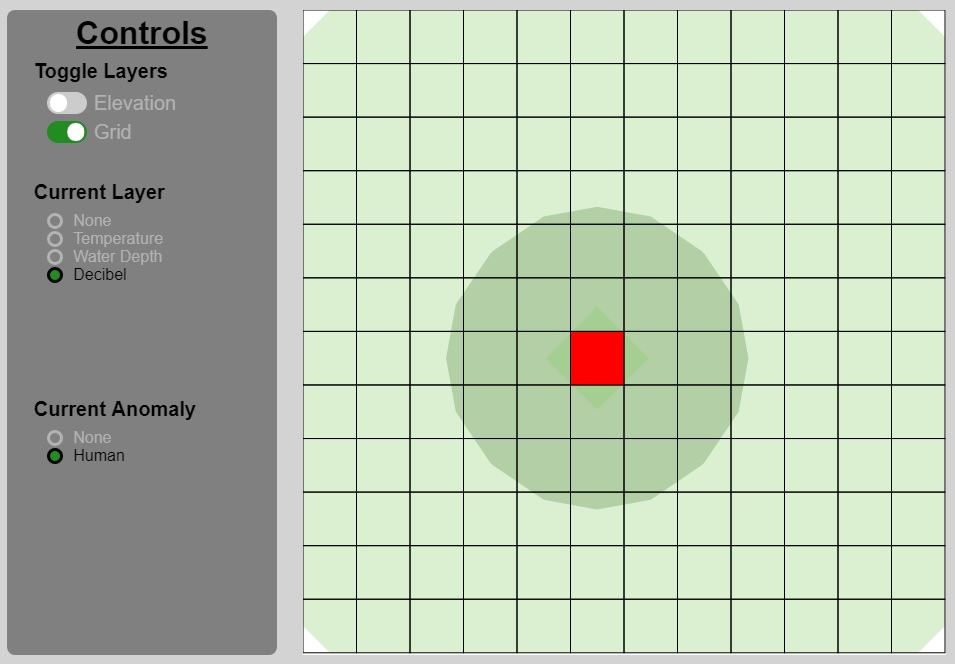
\includegraphics[width=1.0\columnwidth]{Figures/Visualizer/toolbar.JPG}
  \caption[GUI Visualization Toolbar]{Example of the environment-visualizer's toolbar being used to manipulate the display section. The elevation layer has been toggled off, the decibel layer has been selected to be displayed (as a green-scale heatmap), and the human anomaly has been selected and its location is highlighted as the red cell within the display.}
  \label{fig:toolbar}
\end{figure}

\subsubsection{Legend}
The legend provides an overview of the environment in three main subsection: environment, layer and cell.
For the environment subsection, the name of the current environment is displayed along with the dimensions and minimum and maximum elevation within the environment.
The layer subsection displays the minimum and maximum values of the selected display layer (if one is selected), as well as the display layer's value at the selected cell (if a cell is selected).
When a cell is selected, the values of all element types in the area covered by the cell are presented in a list, as well as the cell's relative coordinates in the grid (e.g., figure~\ref{fig:legend}).

\begin{figure}[!htb]
  \centering
  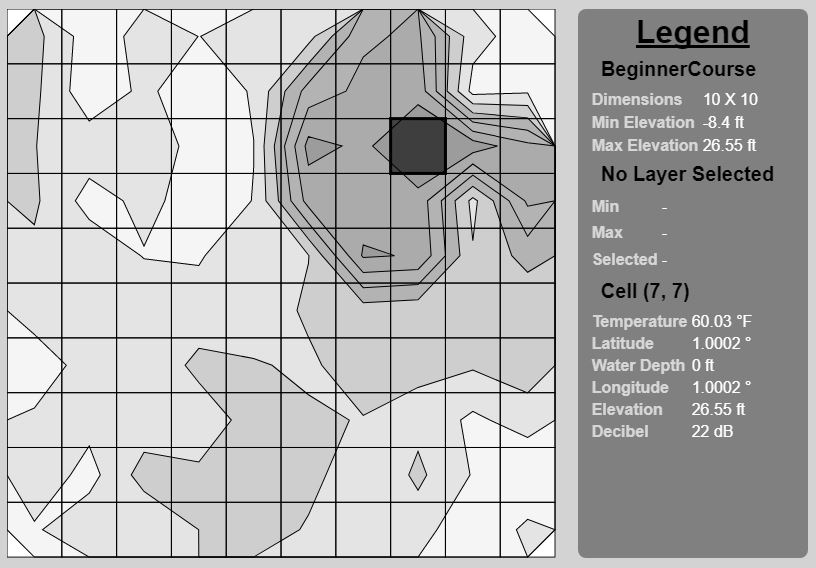
\includegraphics[width=1.0\columnwidth]{Figures/Visualizer/legend.JPG}
  \caption[GUI Visualizer Legend]{Example of the environment-visualizer's legend displaying position and element value information about cell (7, 7) selected from the environment grid (highlighted as a darker shade of grey within the display grid).}
  \label{fig:legend}
\end{figure}

\subsubsection{Operation Log}
The operation log section is a special section that only appears in the visualizer when the user loads an operation run.
This section has buttons that allow the user to step through each event that took place during the given agent's operation (see figure~\ref{fig:operation_controls}).
The user can select to step forward or backwards by 1 or 10 events.
When each event is loaded into the visualizer, the display section will update by selecting the cell where the agent is currently located.
There is also a text display section that shows the index of the event that is currently being viewed, the action that was chosen, the health and energy of the agent during this event, and the long-term and short-term rewards that were received.

\begin{figure}[!htb]
  \centering
  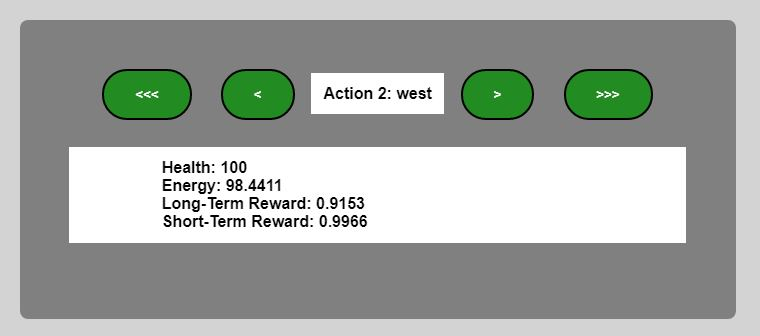
\includegraphics[width=1.0\columnwidth]{Figures/Visualizer/operation_controls.JPG}
  \caption[GUI Operation View Tool]{A command and dialog display tool that will supplement the environment-visualization page when viewing an operation log of an agent. The user can use the ``$\textless\textless\textless$'' and ``$\textless$'' buttons to step backwards 10 and 1 events in the log, and the ``$\textgreater\textgreater\textgreater$'' and ``$\textgreater$'' buttons to step forward 10 and 1 events in the log. The agent's health and energy are displayed during the current event being viewed from the log, along with the action's index within the log, the action selected, and the short-term and long-term rewards that were received for the event.}
  \label{fig:operation_controls}
\end{figure}
